% !TeX_ROOT=../../thesis.tex

%\documentclass[version=final]{iacrcc}
%\usepackage[T1]{fontenc}
%\usepackage{graphicx}
%\usepackage{amssymb}
%\usepackage{amsmath}
%\usepackage{amsthm}
%\usepackage{stmaryrd}
%\usepackage{algorithm, float}
%\usepackage[noend]{algpseudocode}
%\usepackage{array}
%\usepackage{tabularx}
%\usepackage{xcolor}
%\usepackage{bbold}
%\usepackage{subcaption}
%\usepackage{xfrac}
%\usepackage{listings}
%\usepackage{fancyvrb}
%\usepackage{comment}
%\usepackage{algpseudocode}
%\usepackage{algorithm}
%\usepackage{longtable}
%\usepackage{adjustbox}
%\usepackage{lmodern}
%\usepackage{MnSymbol,wasysym}
%\usepackage{enumitem}
%\usepackage{listings}
%\usepackage{tcolorbox}
%%%\usepackage[font=small,skip=0pt]{caption}
%\usepackage{amsthm} % For the environment "primitive"
%\usepackage{pgf,tikz}
%\usepackage{xcolor}
%\usepackage{multirow}
%\usepackage[normalem]{ulem}
%


%
%\begin{abstract}
% Making the most of TFHE advanced capabilities such as programmable or circuit bootstrapping and their generalizations for manipulating data larger than the native plaintext domain of the scheme is a very active line of research. In this context, AES is a particularly interesting benchmark, as an example of a nontrivial algorithm which has eluded ``practical'' FHE execution performances for years, as well as the fact that it will most likely be selected by NIST as a flagship reference in its upcoming call on threshold (homomorphic) cryptography. Since 2023, the algorithm has thus been the subject of a renewed attention from the FHE community and has served as a playground to test advanced operators following the LUT-based, $p$-encodings or several variants of circuit bootstrapping, each time leading to further timing improvements. Still, AES is also interesting as a benchmark because of the tension between boolean- and byte-oriented operations within the algorithm. In this paper, we resolve this tension by proposing a new approach, coined ``\hippo'', which consistently combines the (byte-oriented) LUT-based approach with a generalization of the (boolean-oriented) $p$-encodings one to get the best of both worlds. In doing so, we obtain the best timings so far, getting a \emph{single-core} execution of the algorithm over TFHE from $46$ down to $32$ seconds and approaching the $1$ second barrier with only a mild amount of parallelism. We should also stress that all the timings reported in this paper are consistently obtained on the same machine which is often not the case in previous studies. Lastly, we emphasize that the techniques we develop are applicable beyond just AES since the boolean-byte tension is a recurrent issue when running algorithms over TFHE.
%\end{abstract}
%


%The last example of application of the previous chapter was to evaluate homomorphically the AES cipher.  But why would one want to perform such a computation in the first place?

There are two answers to this question. First,  AES is a particularly interesting benchmark, as an example of a nontrivial algorithm which has eluded ``practical'' FHE execution performances for years. This is part of the reason why it will most likely be selected by NIST as a flagship reference in its upcoming call on threshold (homomorphic) cryptography \cite{call_nist}. Since 2023, the algorithm has thus been the subject of a renewed attention from the FHE community and has served as a playground to test advanced operators\cite{DBLP:conf/wahc/TramaCBS23, ISC:WWLLL23, TCHES:BonPoiRiv24, TCHES:WLWLLW24}. AES is particularly interesting as a benchmark notably because of the tension between boolean- and byte-oriented operations within the algorithm.


There is also a more down-to-earth reason: evaluating symmetric ciphers using FHE is the core of a cryptographic technique called \textit{transciphering}, which is a promising solution for solving the \textit{ciphertext expansion} problem of FHE. In this protocol, the client first encrypts its data using a symmetric encryption scheme and sends both the encrypted data and (once and for all) the FHE-encrypted symmetric key to the server. Leveraging its encrypted-domain computing capabilities, the server can then decrypt the encrypted data \emph{within the homomorphic domain}, ultimately producing homomorphic ciphertexts on which it can perform the requested calculations. With this trick, the amount of data uploaded by the client is drastically reduces, as symmetric ciphertexts are much lighter than homomorphic ones.


In this chapter, we introduce \hippo, the fastest homomorphic implementation of AES using TFHE at the time of writing. To construct it, we leveraged three main ideas:

\begin{itemize}
	\item[-] We generalized the $p$-encoding construction introduced in Chapter \ref{chap:p_encodings} to the arithmetic case.
	\item[-] The LUT-oriented implementation of \cite{DBLP:conf/wahc/TramaCBS23} is very efficient to evaluate the large Sbox of AES, so we borrowed this idea as it was.
	\item[-] We associated both previous techniques by developing a framework of conversion between Boolean and arithmetic representations.
\end{itemize}


The result of this work is doubly interesting: first, we manage to outperform the rest of the literature on homomorphic AES evaluation. Second, we develop a generic framework useful to resolve the recurring tension between Boolean and arithmetic representations within homomorphic circuits, which we believe is of independent interest.


We start this chapter by introducing the notion of transciphering in Section \ref{sec:transciphering}, which will be a recurring theme in the rest of this manuscript. Then, after some preliminaries on the AES cipher (Section \ref{sec:preliminaries_aes}), we introduce in Section \ref{sec:previous-blocks} some advanced homomorphic operators from \cite{DBLP:conf/wahc/TramaCBS23} that will be useful in this work. We then generalize the $p$-encoding construction of Chapter \ref{chap:p_encodings} to the arithmetic case (Section \ref{sec:generalization_p_encodings}). Finally, Section~\ref{sec:hippogryph_our_work} introduces our new design and Section~\ref{sec:comparison} presents a detailed comparison with existing approaches, supported by relevant benchmarks.


\TODO{Mettre la table récapitulative du papier ici ?}



\TODO{Retravailler l'introduction et la mettre ici. Merger avec l'abstract}
 % !TeX_ROOT=../../thesis.tex
 
\section{Preliminaries on AES}
\label{sec:preliminaries_aes}

The Advanced Encryption Standard (AES), based on the Rijndael algorithm winner of the NIST competition in 2000 \cite{aes-original}, is a symmetric block cipher supporting key sizes of 128, 192, and 256 bits. Depending on the key size, AES uses 10, 12, or 14 rounds of processing, each applying a fixed sequence of substitution, permutation, and mixing steps to transform plaintext into ciphertext (or ciphertext into plaintext for decryption). A key schedule generates round keys for each encryption round, plus an initial key.

\hippo focuses on AES with 128-bit keys, which uses 10 rounds. The encryption begins with an \AddRoundKey step, followed by 10 rounds. Each round includes four steps: \SubBytes, \ShiftRows, \MixColumns, and \AddRoundKey, except the final round, which omits \MixColumns. Below, we recall the key expansion and the subroutines:
\begin{itemize}
\item \texttt{Key Expansion}: The \texttt{Key Expansion} operation is performed once for a given secret key. Starting from the 128-bit key (in our context), it generates eleven 128-bit round keys, which are then used in the \AddRoundKey operation throughout the AES encryption or decryption process, without needing access to the original key. The key expansion involves XORs and $\F_{256}$ multiplications.

    \item \SubBytes: The \SubBytes operation is the only non-linear transformation in the cipher. It involves a substitution step, where each byte in the state matrix is replaced according to a fixed S-box. Since it operates independently on each byte of the state, \SubBytes can be easily parallelized, allowing for more efficient execution.
    \item \AddRoundKey: 
    %Before encryption begins, the secret key undergoes an "expansion" process to generate several round keys. The encryption procedure relies solely on these round keys, rather than the initial secret key. 
    During this transformation, the state is updated by combining it with the current round key using a bitwise XOR operation. Specifically, the 128-bit round key is organized into a matrix format to align with the structure of the state matrix, and the two matrices are XORed element-wise to produce the new state.
   
    \item \ShiftRows: The \ShiftRows step is a byte transposition that cyclically shifts the rows of the state by different offsets. For AES with 128-bit keys, the first row remains unchanged, the second row is shifted by one byte, the third by two bytes, and the fourth row by three bytes. 

    \item \MixColumns: The \MixColumns step processes the state column by column through matrix multiplication. To compute each byte of the state matrix, they combine scalar multiplication in $\mathtt{GF}(256)$ with XOR operations. This approach facilitates parallelization of the operation.  
    
    
\end{itemize}


\TODO{Splitter la section suivante entre des préliminaires sur les PBS tweakée et la généralisation des p-encodings}

\section{Some Building Blocks for LUT-based Evaluation}
\label{sec:previous-blocks}


In this section, we present the approach from \cite{DBLP:conf/wahc/TramaCBS23}, some components of which we use for our own work. We formally present some advanced homomorphic primitives used in this work that we reuse as well.


\cite{DBLP:conf/wahc/TramaCBS23} is a ``Full-LUT'' approach, that is to say AES is evaluated entirely with TFHE's programmable bootstrapping, encoding exclusively all operations within LUTs. To meet the performance constraints of the bootstrapping algorithm, this method operates on elements in $\Z_{16}$, ensuring efficient computation.

\subsection{AES Subroutines as LUTs}

The \SubBytes step, which involves the evaluation of an S-box, is inherently a LUT operation and is therefore naturally implemented in FHE using a PBS. However, PBS is too slow in $\F_{256}$ (as we have seen in Section \ref{sec:pbs_performances}). So, they rely on a construction evaluating PBS over $\Z_{16}$ rather than $\F_{256}$. Moreover, converting the other AES steps into LUT evaluations also requires additional effort.

In particular, in the original AES design \cite{aes-original}, the \MixColumns step is computed using a series of XOR operations and multiplications in $\F_{256}$. Unfortunately, TFHE’s native multiplication \texttt{ClearMultTFHE} cannot directly handle these $\F_{256}$ multiplications because of the polynomial nature of the elements of this field. As a result, \MixColumns must be reformulated as a LUT evaluation.

Additionally, the \AddRoundKey step, which uses XOR as its key operation, presents its own challenges because XOR is a bivariate operation that requires two inputs. Classical bootstrapping, which operates on single inputs, is insufficient for this purpose. To address this, the authors utilize a specialized bootstrapping method that supports operations on multiple encrypted inputs.

\subsection{LUTs Evaluation} 
Since the AES evaluation involves computing an 8-bit S-box, a straightforward solution would be to work with 8-bit messages. With such messages, the homomorphic S-box evaluation would require only one bootstrapping per byte. However, processing messages with more bits significantly slow down the bootstrapping process. To address this issue, \cite{DBLP:conf/wahc/TramaCBS23} proposes a decomposition approach and demonstrates that the optimal representation of 8-bit inputs for their purpose is in $\Z_{16}$. Specifically, a message $m \in \{0, \cdots, 255\}$ is split into two 4-bit chunks (or \emph{nibbles}) $h$ and $l$ such that $m = 16h+l$. The encryption of $m$ is then represented as two ciphertexts encrypting $h$ and $l$ with the same key $\lweSecretKey$.

However, bootstrapping these decomposed inputs requires a method capable of handling multiple encrypted inputs. The authors explore several approaches for this, namely the chain-based method and the tree-based method \cite{TCHES:GuiBorAra21}. Their analysis concludes that the Tree-Based Method (TBM) is the most suitable for their needs. They also relies on the Multi-Value Bootstrapping (MVB) to produce several outputs for the cost of one PBS. We provide details about TBM and MVB in the following:

\paragraph{Multi-Value Bootstrapping from \cite{RSA:CarIzaMol19}.}
\label{primitive:mvb}
%
Multi-Value Bootstrapping (MVB) is a technique that enables the evaluation of $k$ distinct Look-Up Tables $(f_i)_{1 \le i \le k}$ on a single encrypted input, using only one $\BlindRotate$. This method is based on the factorization of the accumulator polynomials $\textsf{acc}_i(X)$ associated with each function $f_i$. Specifically, each accumulator polynomial is expressed as: 
$$
    \textsf{acc}_i(X) = \sum_{j=0}^{N-1} \alpha_{i,j} X^j, \quad \alpha_{i,j} \in \mathbb{Z}_q.
$$
The factorization then splits it into two parts: 
$$
    \textsf{acc}_i(X) = v_0(X) \cdot v_i(X) \mod (X^N + 1),
$$
where $v_0(X)$ is a common factor shared across all accumulators set as:
$$
    v_0(X) = \frac{1}{2} \cdot (1 + X + \dots + X^{N-1}),
$$
and $v_i(X)$ is a distinct factor specific to each function $f_i$:
$$
    v_i(X) = \alpha_{i, 0} + \alpha_{i, N-1} + (\alpha_{i, 1} - \alpha_{i, 0}) \cdot X + \dots + (\alpha_{i, N-1} - \alpha_{i, N-2}) \cdot X^{N-1}.
$$
This factorization is made possible thanks to the identity:
$$
(1 + X + \dots + X^{N-1}) \cdot (1-X) \equiv 2 \mod (X^N + 1).
$$
By leveraging this factorization and as illustrated on Figure~\ref{fig:mvb}, multiple LUTs can be evaluated on a single encrypted input by performing the following steps:
\begin{enumerate}
\item Computing a $\BlindRotate$ operation on an accumulator polynomial initialized with the value of $v_0$.
\item Then multiplying with \texttt{ClearMultTFHE} the obtained rotated polynomial by each $v_i(X)$ corresponding to the LUT of $f_i$ to obtain the respective $\textsf{acc}_i(X)$.
\end{enumerate}
Finally, at the cost of a single $\BlindRotate$ and $k$ \texttt{clearMultTFHE} operations (on $\GLWE$), one can obtain the evaluation of $k$ different LUTs on one single encrypted input. Moreover, this specific choice of factorization allows for a very-low norm for the vectors $v_i$'s (which in practice are very sparse), and so a very-low noise expansion.

\begin{figure}
	\centering
	\begin{subfigure}[t]{\linewidth}
		\centering
		\mvbFigureA % <-- Replace with your TikZ or figure content
		\caption{Classic bootstrapping method to evaluate several LUTs on a single input}
		\label{fig:mvbA}
	\end{subfigure}
	
	\vspace{1.5em} % vertical space between figures
	
	\begin{subfigure}[t]{\textwidth}
		\centering
		\mvbFigureB % <-- Replace with your TikZ or figure content
		\caption{MVB method}
		\label{fig:mvbB}
	\end{subfigure}
	
	\caption{Difference between the classical approach and the MVB. Pink arrows represent \texttt{clearMultTFHE} operations (on $\GLWE$).}
	\label{fig:mvb}
\end{figure}

This MVB primitive thus allows significant speed-ups in the implementation of \cite{DBLP:conf/wahc/TramaCBS23}, in particular in the evaluation of the S-box or in the multiplications in $\F_{256}$ that occur during the \MixColumns step. Indeed, since each byte is decomposed into two nibbles $h$ and $l$, the LUT corresponding, for instance, to the S-box must also be decomposed into two tables: one providing the most significant nibble and one providing the least significant nibble. That is to say: 
$$
\texttt{tab}_{\textsc{msn}}[i] = \left\lfloor \frac{\texttt{S-box}[i]}{16} \right\rfloor \quad \text{and} \quad \texttt{tab}_{\textsc{lsn}}[i] = \texttt{S-box}[i] \mod 16.
$$
Each of these tables must be evaluated on an 8-bit payload ciphertext. 


\paragraph{Tree-Based Method from \cite{DBLP:conf/wahc/TramaCBS23}.}
\label{prim:tbb}

Let $B, B', d \in \mathbb N^*$. The Tree-Based Method (TBM) allows to evaluate a LUT $f: \Z_{B^d} \mapsto \Z_ {B'}$ with a large input size $B^d$, by processing $d$ limbs of data in $\Z_B$. We consider input messages that are written as:
$$
    m = \sum_{i=0}^{d-1} m_i B^i, \quad \text{with } m_i \in \mathbb{Z}_B,
$$
and that are represented by $d$ ciphertexts $(\vec c_0, \vec c_1, \dots, \vec c_{d-1})$ corresponding to the $d$ message components $(m_0, m_1, \dots, m_{d-1})$. 
%
To evaluate $f$, we encode a LUT for $f$ using $B^{d-1}$ accumulators, each represented by a polynomial $\textsf{acc}_i(X)$. These accumulators encode the functions:
%
    \begin{align*}
        f_i: \Z_B &\rightarrow \Z_{B'}\\
             x &\mapsto f(i + x \cdot B^{d-1})
    \end{align*}
%
Next, we apply a $\sf{BlindRotate}$ and a $\sf{SampleExtract}$ to each accumulator $\textsf{acc}_i(X)$, using $\vec c_{d-1}$ as the selector. This operation produces $B^{d-1}$ LWE ciphertexts, each encrypting $f (i + m_{d-1} \cdot B^{d-1})$ for $i \in \Z_{B^{d-1}}$.
%    
Finally, a $\sf{Keyswitch}$ operation from LWE to GLWE aggregates these ciphertexts into $B^{d-2}$ GLWE encryptions, representing the LUT of $h$, defined as:
    \begin{align*}
        h &: (\Z_{B})^{d-1} \mapsto \Z_B' \\
          & (u_0, \dots, u_{d-1}) \mapsto f \circ g(u_0, \dots, u_{d-2}, m_{d-1})
    \end{align*}
using the bijection $g$, which reverses the decomposition:
    \begin{align*}
        g: (\Z_B)^d &\rightarrow \Z_{B^d} \\
           (u_0, \dots, u_{d-1}) &\mapsto \sum_{i=0}^{d-1} u_i \cdot B^i
    \end{align*} 

This process is repeated iteratively, using the next ciphertext at each step, until a single LWE ciphertext encrypting $f(m_0, \dots, m_{d-1})$ is obtained.  


\begin{figure}
    \centering
    \treePBSFigure
    \caption{Illustration of the tree-based method on messages  $m_1 = 1, m_2=2$ in the space  $\mathbb{Z}_4$. The corresponding ciphertexts are $\vec c_1 \in \LWE(m_1)$ and $\vec c_2 \in \LWE(m_2)$. We apply the addition in $\mathbb{Z}_4$ via programmable bootstrapping. Red arrows indicate bootstrappings. (Figure inspired by \cite{DBLP:conf/wahc/TramaCBS23}.)}
    \label{fig:my_label}
\end{figure}

In the implementation described in \cite{DBLP:conf/wahc/TramaCBS23}, this primitive is employed to evaluate an 8-bit LUT by dividing it into two limbs of 4 bits each, which they determined to be optimal for their specific setting. 
%
To further enhance the performance of the TBM, the blind rotations for the accumulators $acc_i(X)$ of \emph{the first layer of the tree} can be performed simultaneously using the MVB technique (as discussed in~\cite{TCHES:GuiBorAra21}). 

Finally, the ``full-LUT'' approach facilitates efficient computation of the S-box through the Tree-Based Method, as opposed to directly evaluating the corresponding Boolean circuit. However, this approach also requires LUT-based computation of XOR operations and other intermediary steps, which is notably slower when operating in $\Z_{16}$ compared to binary messages. Consequently, our new method \hippo{} proposed in this chapter strategically applies LUT evaluation exclusively where it is most effective and yields the best performance, namely for the evaluation of the S-box.




\section{Generalization of $p$-encodings to Arithmetic Case}
\label{sec:generalization_p_encodings}

In Chapter \ref{chap:p_encodings} of this thesis, we introduced the notion of $p$-encodings and used it in Section \ref{sec:p_encodings_aes} to evaluate AES homomorphically. In this method, data was encrypted bit per bit and only Boolean operations were performed. It leveraged the fact that, in the plaintext space $\Z_2$, the \texttt{SumTFHE} operation actually performs a XOR. Thus, the linear operations \MixColumns and \AddRoundKey could be efficiently performed with minimal cost, using only the homomorphic sum of TFHE. To be able to evaluate $\SubBytes$ under Boolean representation, we used $p$-encodings to evaluate the circuits of \SubBytes with a minimal number of bootstrappings. While this has brought some improvements, evaluating the LUT of AES as a Boolean circuit is still suboptimal, and in this chapter we attempt at doing it using arithmetic representation.

To achieve that, we generalize $p$-encodings beyond the Boolean case by defining the $(o, p)$- encoding construction. Informally, instead of embedding the Boolean space in $\Z_p$, we embed any space $\Z_o$ in $\Z_p$ (with $o < p$). So, what was called $p$-encoding in Chapter \ref{chap:p_encodings} corresponds to a $(2, p)$-encoding in this one.
%
Definition \ref{def:encoding} formalizes this generalization.

\begin{definition}[$(o, p)$-encoding]
	Let $\Z_o$ be the message space. A \emph{$(o, p)$-encoding} is a function $\Encoding: \Z_o \mapsto 2^{\Z_p}$ that maps each element of $\Z_o$ to a subset of the discretized torus $\Z_p$. A $(o, p)$-encoding is \emph{valid} if and only if:
	\begin{equation}
		\begin{cases}
			\forall (i, j) \in \Z_o^2, i \ne j, \Encoding(i) \cap \Encoding(j) = \emptyset~\text{ and}\\
			\text{if $p$ is even:} ~\forall \:x \in \mathbb Z_p, \forall i \in \Z_o: x \in \Encoding(i) \iff \left [ x + \frac p 2 \right ]_p \in \Encoding([-i]_o)
		\end{cases}
		\label{def:validity}
	\end{equation}
	The latter property is a direct consequence of the negacyclicity problem, which we discussed extensively in Chapter \ref{chap:negacyclicity}.
	\label{def:encoding}
\end{definition}

In this work, we focus exclusively on cases where $p=2$ or $p$ is an odd prime. As a result, a lot of the subleties of negacyclicity can be overlooked. Furthermore, among the various types of $(o, p)$-encodings, one particular class proves especially useful for our purposes: the \textit{canonical} $(o, p)$-encoding.

\begin{definition}[canonical $(o, p)$-encoding]
	\label{def:canonical-encoding}
	A $(o, p)$-encoding $\Encoding$ is said \textit{canonical} if and only if it verifies: 
	\begin{align*}
		\Encoding: \Z_o &\rightarrow \Z_p\\
		x &\mapsto x
	\end{align*}
	(with $o < p$). Informally, we simply embed a smaller space into a larger one, without altering the order of the elements.
\end{definition}


In Chapter \ref{chap:p_encodings} the Boolean space is used (so $o=2$). The \SubBytes circuit is evaluated using $(2,11)$-encoding, while the rest is evaluated with a $(2, 2)$-encoding (\ie~the trivial encoding of TFHE with plaintext space $\Z_2$). Consequently, an \textit{Encoding Switching} operation is required. This operation can be straightforwardly performed using a PBS.

\begin{definition}[Encoding Switching]
	\label{def:encoding-switching}
	Let $\vec c$ be a ciphertext encrypting a message $m \in \Z_o$ under the $(o, p)$-encoding $\Encoding$. Its encoding can be switched to the $(o, p')$-encoding $\Encoding'$ by applying a PBS on $\vec c$ evaluating the function:
	
	\begin{align*}
		\texttt{Cast}_{\Encoding \mapsto \Encoding'}: \Z_p &\rightarrow \Z_{p'}\\
		x &\mapsto x'
	\end{align*}
	where $x'$ is defined as $\forall i \in \Z_o, x \in \Encoding(i) \implies x' \in \Encoding'(i)$.
\end{definition}



\section{Design of \hippo}
\label{sec:hippogryph_our_work}

Building on the foundation of the two previous works, we develop a hybrid approach, \hippo, that not only combines their respective strengths but also introduces new contributions to enable their effective integration. The guiding principles of this design are outlined below:

\begin{itemize}
    \item The \SubBytes step, which was the weak point of \cite{TCHES:BonPoiRiv24}, is evaluated using the strategy of \cite{DBLP:conf/wahc/TramaCBS23}.
    \item Conversely, the linear steps (namely \ShiftRows, \MixColumns and \AddRoundKey) are computed using a trivial $(2, 2)$-encoding, which makes them extremely fast.
    \item Since the two aforementioned points rely on different data representations (arithmetic for \SubBytes and Boolean for the other steps), a decomposition layer and a recomposition layer are necessary to transition from one to another. The decomposition and recomposition steps are denoted by \texttt{Decomposer} and \texttt{Recomposer}, respectively. %To make them work, we make use of a $(o, p)$-encoding for the \SubBytes step. This will be explained in further details in this section.
\end{itemize}

Our design for one round of AES is summed up on \ref{fig:our_design}. In the following we explain each of its components.

\usetikzlibrary{arrows}
\begin{figure}
	\centering
      \definecolor{qqttff}{rgb}{0,0.2,1}
\definecolor{fffftt}{rgb}{0.9,0.9,0.2}
\definecolor{ffffqq}{rgb}{0.9,0.9,0}
\definecolor{ttttff}{rgb}{0.2,0.2,1}
\definecolor{zzttqq}{rgb}{0.6,0.2,0}
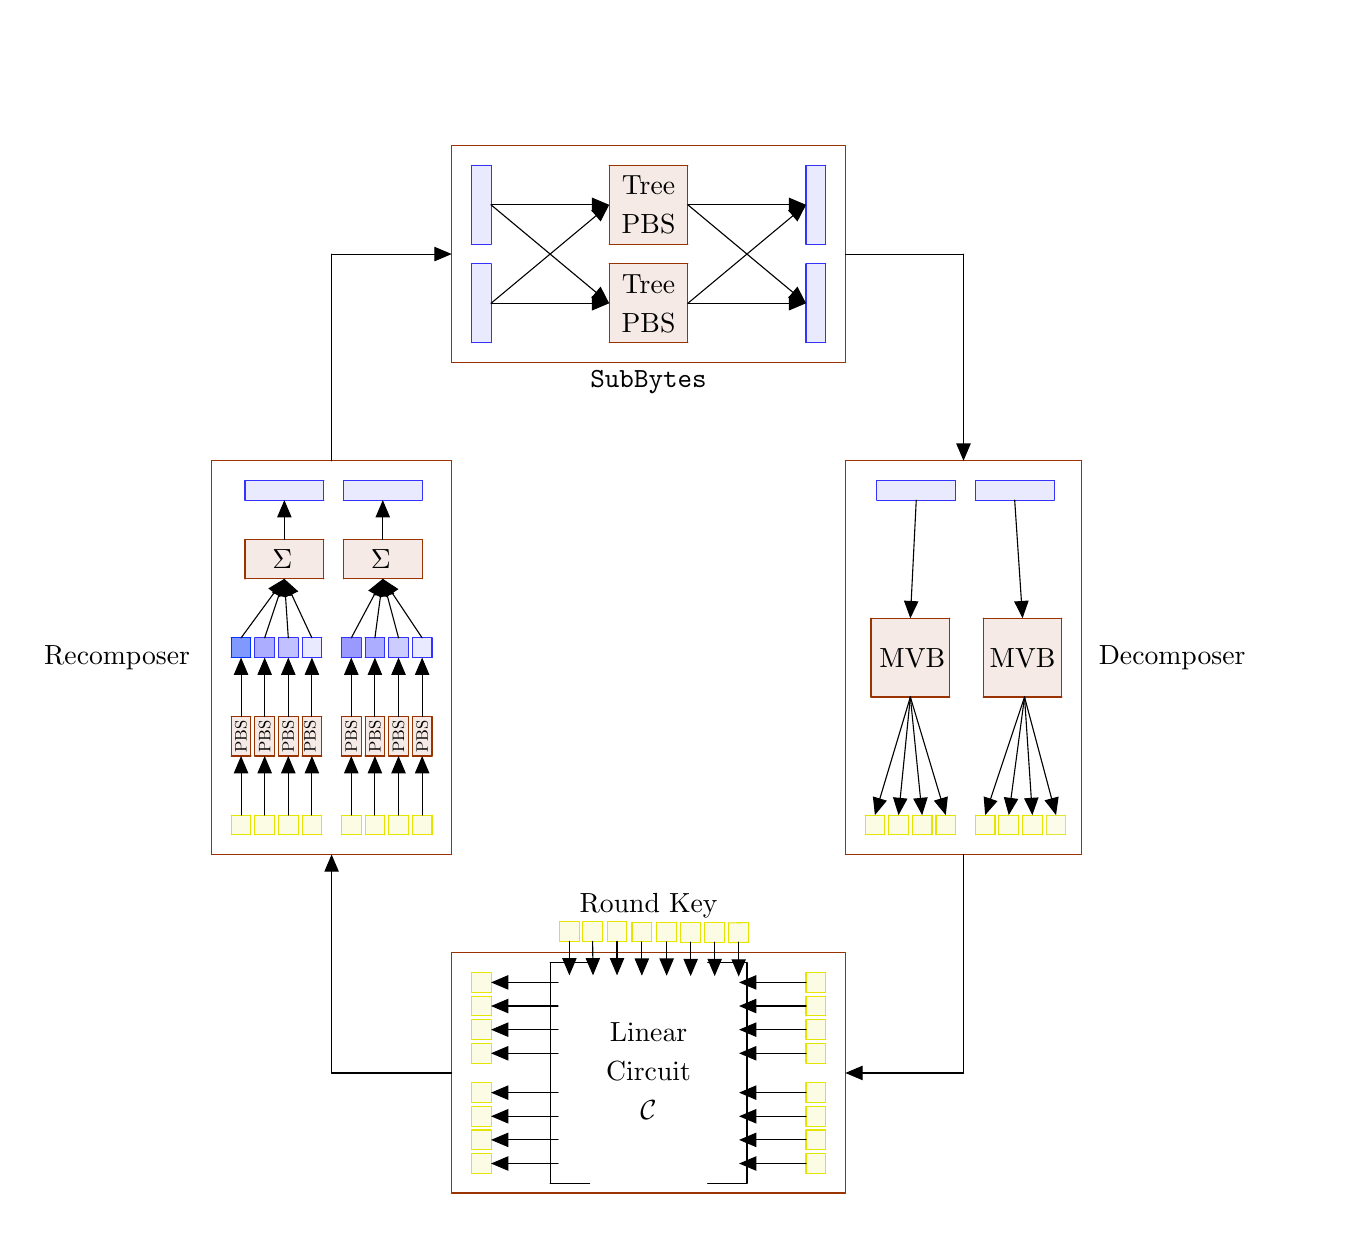
\begin{tikzpicture}[line cap=round,line join=round,>=triangle 45,x=0.5cm,y=0.5cm]
\clip(-10.77,-27) rectangle (22,3);
\fill[color=ttttff,fill=ttttff,fill opacity=0.1] (0.5,-0.5) -- (1,-0.5) -- (1,-2.5) -- (0.5,-2.5) -- cycle;
\fill[color=ttttff,fill=ttttff,fill opacity=0.1] (0.5,-3) -- (1,-3) -- (1,-5) -- (0.5,-5) -- cycle;
\fill[color=zzttqq,fill=zzttqq,fill opacity=0.1] (4,-0.5) -- (6,-0.5) -- (6,-2.5) -- (4,-2.5) -- cycle;
\fill[color=zzttqq,fill=zzttqq,fill opacity=0.1] (4,-3) -- (6,-3) -- (6,-5) -- (4,-5) -- cycle;
\fill[color=ttttff,fill=ttttff,fill opacity=0.1] (9,-0.5) -- (9.5,-0.5) -- (9.5,-2.5) -- (9,-2.5) -- cycle;
\fill[color=ttttff,fill=ttttff,fill opacity=0.1] (9,-3) -- (9.5,-3) -- (9.5,-5) -- (9,-5) -- cycle;
\fill[color=ttttff,fill=ttttff,fill opacity=0.1] (10.8,-8.5) -- (12.8,-8.5) -- (12.8,-9) -- (10.8,-9) -- cycle;
\fill[color=ttttff,fill=ttttff,fill opacity=0.1] (13.3,-8.5) -- (15.3,-8.5) -- (15.3,-9) -- (13.3,-9) -- cycle;
\fill[color=ffffqq,fill=ffffqq,fill opacity=0.1] (10.5,-17) -- (11,-17) -- (11,-17.5) -- (10.5,-17.5) -- cycle;
\fill[color=ffffqq,fill=ffffqq,fill opacity=0.1] (11.1,-17) -- (11.6,-17) -- (11.6,-17.5) -- (11.1,-17.5) -- cycle;
\fill[color=ffffqq,fill=ffffqq,fill opacity=0.1] (11.7,-17) -- (12.2,-17) -- (12.2,-17.5) -- (11.7,-17.5) -- cycle;
\fill[color=ffffqq,fill=ffffqq,fill opacity=0.1] (12.3,-17) -- (12.8,-17) -- (12.8,-17.5) -- (12.3,-17.5) -- cycle;
\fill[color=ffffqq,fill=ffffqq,fill opacity=0.1] (13.3,-17) -- (13.8,-17) -- (13.8,-17.5) -- (13.3,-17.5) -- cycle;
\fill[color=ffffqq,fill=ffffqq,fill opacity=0.1] (13.9,-17) -- (14.4,-17) -- (14.4,-17.5) -- (13.9,-17.5) -- cycle;
\fill[color=ffffqq,fill=ffffqq,fill opacity=0.1] (14.5,-17) -- (15,-17) -- (15,-17.5) -- (14.5,-17.5) -- cycle;
\fill[color=fffftt,fill=fffftt,fill opacity=0.1] (15.1,-17) -- (15.6,-17) -- (15.6,-17.5) -- (15.1,-17.5) -- cycle;
\fill[color=zzttqq,fill=zzttqq,fill opacity=0.1] (10.65,-12) -- (12.65,-12) -- (12.65,-14) -- (10.65,-14) -- cycle;
\fill[color=zzttqq,fill=zzttqq,fill opacity=0.1] (13.5,-12) -- (15.5,-12) -- (15.5,-14) -- (13.5,-14) -- cycle;
\fill[color=ffffqq,fill=ffffqq,fill opacity=0.1] (-5.6,-17) -- (-5.1,-17) -- (-5.1,-17.5) -- (-5.6,-17.5) -- cycle;
\fill[color=ffffqq,fill=ffffqq,fill opacity=0.1] (-5,-17) -- (-4.5,-17) -- (-4.5,-17.5) -- (-5,-17.5) -- cycle;
\fill[color=ffffqq,fill=ffffqq,fill opacity=0.1] (-4.4,-17) -- (-3.9,-17) -- (-3.9,-17.5) -- (-4.4,-17.5) -- cycle;
\fill[color=ffffqq,fill=ffffqq,fill opacity=0.1] (-3.8,-17) -- (-3.3,-17) -- (-3.3,-17.5) -- (-3.8,-17.5) -- cycle;
\fill[color=ffffqq,fill=ffffqq,fill opacity=0.1] (-2.8,-17) -- (-2.3,-17) -- (-2.3,-17.5) -- (-2.8,-17.5) -- cycle;
\fill[color=ffffqq,fill=ffffqq,fill opacity=0.1] (-2.2,-17) -- (-1.7,-17) -- (-1.7,-17.5) -- (-2.2,-17.5) -- cycle;
\fill[color=ffffqq,fill=ffffqq,fill opacity=0.1] (-1.6,-17) -- (-1.1,-17) -- (-1.1,-17.5) -- (-1.6,-17.5) -- cycle;
\fill[color=ffffqq,fill=ffffqq,fill opacity=0.1] (-1,-17) -- (-0.5,-17) -- (-0.5,-17.5) -- (-1,-17.5) -- cycle;
\fill[color=zzttqq,fill=zzttqq,fill opacity=0.1] (-5.6,-14.5) -- (-5.1,-14.5) -- (-5.1,-15.5) -- (-5.6,-15.5) -- cycle;
\fill[color=zzttqq,fill=zzttqq,fill opacity=0.1] (-5,-14.5) -- (-4.5,-14.5) -- (-4.5,-15.5) -- (-5,-15.5) -- cycle;
\fill[color=zzttqq,fill=zzttqq,fill opacity=0.1] (-4.4,-14.5) -- (-3.9,-14.5) -- (-3.9,-15.5) -- (-4.4,-15.5) -- cycle;
\fill[color=zzttqq,fill=zzttqq,fill opacity=0.1] (-3.8,-14.5) -- (-3.3,-14.5) -- (-3.3,-15.5) -- (-3.8,-15.5) -- cycle;
\fill[color=zzttqq,fill=zzttqq,fill opacity=0.1] (-2.8,-14.5) -- (-2.3,-14.5) -- (-2.3,-15.5) -- (-2.8,-15.5) -- cycle;
\fill[color=zzttqq,fill=zzttqq,fill opacity=0.1] (-2.2,-14.5) -- (-1.7,-14.5) -- (-1.7,-15.5) -- (-2.2,-15.5) -- cycle;
\fill[color=zzttqq,fill=zzttqq,fill opacity=0.1] (-1.6,-14.5) -- (-1.1,-14.5) -- (-1.1,-15.5) -- (-1.6,-15.5) -- cycle;
\fill[color=zzttqq,fill=zzttqq,fill opacity=0.1] (-1,-14.5) -- (-0.5,-14.5) -- (-0.5,-15.5) -- (-1,-15.5) -- cycle;
\fill[color=qqttff,fill=qqttff,fill opacity=0.5] (-5.6,-12.5) -- (-5.1,-12.5) -- (-5.1,-13) -- (-5.6,-13) -- cycle;
\fill[color=ttttff,fill=ttttff,fill opacity=0.3] (-4.4,-12.5) -- (-3.9,-12.5) -- (-3.9,-13) -- (-4.4,-13) -- cycle;
\fill[color=ttttff,fill=ttttff,fill opacity=0.4] (-5,-12.5) -- (-4.5,-12.5) -- (-4.5,-13) -- (-5,-13) -- cycle;
\fill[color=ttttff,fill=ttttff,fill opacity=0.1] (-3.8,-12.5) -- (-3.3,-12.5) -- (-3.3,-13) -- (-3.8,-13) -- cycle;
\fill[color=ttttff,fill=ttttff,fill opacity=0.5] (-2.8,-12.5) -- (-2.3,-12.5) -- (-2.3,-13) -- (-2.8,-13) -- cycle;
\fill[color=ttttff,fill=ttttff,fill opacity=0.4] (-2.2,-12.5) -- (-1.7,-12.5) -- (-1.7,-13) -- (-2.2,-13) -- cycle;
\fill[color=ttttff,fill=ttttff,fill opacity=0.25] (-1.6,-12.5) -- (-1.1,-12.5) -- (-1.1,-13) -- (-1.6,-13) -- cycle;
\fill[color=ttttff,fill=ttttff,fill opacity=0.1] (-1,-12.5) -- (-0.5,-12.5) -- (-0.5,-13) -- (-1,-13) -- cycle;
\fill[color=zzttqq,fill=zzttqq,fill opacity=0.1] (-5.25,-10) -- (-3.25,-10) -- (-3.25,-11) -- (-5.25,-11) -- cycle;
\fill[color=zzttqq,fill=zzttqq,fill opacity=0.1] (-2.75,-10) -- (-0.75,-10) -- (-0.75,-11) -- (-2.75,-11) -- cycle;
\fill[color=ttttff,fill=ttttff,fill opacity=0.1] (-5.25,-8.5) -- (-3.25,-8.5) -- (-3.25,-9) -- (-5.25,-9) -- cycle;
\fill[color=ttttff,fill=ttttff,fill opacity=0.1] (-2.75,-8.5) -- (-0.75,-8.5) -- (-0.75,-9) -- (-2.75,-9) -- cycle;
\fill[color=ffffqq,fill=ffffqq,fill opacity=0.1] (0.5,-21) -- (1,-21) -- (1,-21.5) -- (0.5,-21.5) -- cycle;
\fill[color=ffffqq,fill=ffffqq,fill opacity=0.1] (0.5,-21.6) -- (1,-21.6) -- (1,-22.1) -- (0.5,-22.1) -- cycle;
\fill[color=ffffqq,fill=ffffqq,fill opacity=0.1] (0.5,-22.2) -- (1,-22.2) -- (1,-22.7) -- (0.5,-22.7) -- cycle;
\fill[color=ffffqq,fill=ffffqq,fill opacity=0.1] (0.5,-22.8) -- (1,-22.8) -- (1,-23.3) -- (0.5,-23.3) -- cycle;
\fill[color=ffffqq,fill=ffffqq,fill opacity=0.1] (0.5,-23.8) -- (1,-23.8) -- (1,-24.3) -- (0.5,-24.3) -- cycle;
\fill[color=ffffqq,fill=ffffqq,fill opacity=0.1] (0.5,-24.4) -- (1,-24.4) -- (1,-24.9) -- (0.5,-24.9) -- cycle;
\fill[color=ffffqq,fill=ffffqq,fill opacity=0.1] (0.5,-25) -- (1,-25) -- (1,-25.5) -- (0.5,-25.5) -- cycle;
\fill[color=ffffqq,fill=ffffqq,fill opacity=0.1] (0.5,-25.6) -- (1,-25.6) -- (1,-26.1) -- (0.5,-26.1) -- cycle;
\fill[color=ffffqq,fill=ffffqq,fill opacity=0.1] (9,-23.8) -- (9.5,-23.8) -- (9.5,-24.3) -- (9,-24.3) -- cycle;
\fill[color=ffffqq,fill=ffffqq,fill opacity=0.1] (9,-24.4) -- (9.5,-24.4) -- (9.5,-24.9) -- (9,-24.9) -- cycle;
\fill[color=ffffqq,fill=ffffqq,fill opacity=0.1] (9,-25) -- (9.5,-25) -- (9.5,-25.5) -- (9,-25.5) -- cycle;
\fill[color=ffffqq,fill=ffffqq,fill opacity=0.1] (9,-25.6) -- (9.5,-25.6) -- (9.5,-26.1) -- (9,-26.1) -- cycle;
\fill[color=ffffqq,fill=ffffqq,fill opacity=0.1] (9,-23.3) -- (9.5,-23.3) -- (9.5,-22.8) -- (9,-22.8) -- cycle;
\fill[color=ffffqq,fill=ffffqq,fill opacity=0.1] (9,-22.7) -- (9.5,-22.7) -- (9.5,-22.2) -- (9,-22.2) -- cycle;
\fill[color=ffffqq,fill=ffffqq,fill opacity=0.1] (9,-22.1) -- (9.5,-22.1) -- (9.5,-21.6) -- (9,-21.6) -- cycle;
\fill[color=ffffqq,fill=ffffqq,fill opacity=0.1] (9,-21.5) -- (9.5,-21.5) -- (9.5,-21) -- (9,-21) -- cycle;
\fill[color=ffffqq,fill=ffffqq,fill opacity=0.1] (2.74,-19.71) -- (3.24,-19.71) -- (3.24,-20.21) -- (2.74,-20.21) -- cycle;
\fill[color=ffffqq,fill=ffffqq,fill opacity=0.1] (3.33,-19.71) -- (3.83,-19.71) -- (3.83,-20.21) -- (3.33,-20.21) -- cycle;
\fill[color=ffffqq,fill=ffffqq,fill opacity=0.1] (3.95,-19.71) -- (4.45,-19.71) -- (4.45,-20.21) -- (3.95,-20.21) -- cycle;
\fill[color=ffffqq,fill=ffffqq,fill opacity=0.1] (4.58,-19.72) -- (5.08,-19.72) -- (5.08,-20.22) -- (4.58,-20.22) -- cycle;
\fill[color=ffffqq,fill=ffffqq,fill opacity=0.1] (5.21,-19.72) -- (5.71,-19.72) -- (5.71,-20.22) -- (5.21,-20.22) -- cycle;
\fill[color=ffffqq,fill=ffffqq,fill opacity=0.1] (5.82,-19.73) -- (6.32,-19.73) -- (6.32,-20.23) -- (5.82,-20.23) -- cycle;
\fill[color=ffffqq,fill=ffffqq,fill opacity=0.1] (6.43,-19.73) -- (6.93,-19.73) -- (6.93,-20.23) -- (6.43,-20.23) -- cycle;
\fill[color=ffffqq,fill=ffffqq,fill opacity=0.1] (7.02,-19.74) -- (7.55,-19.73) -- (7.55,-20.23) -- (7.02,-20.24) -- cycle;
\draw [color=zzttqq] (0,0)-- (10,0);
\draw [color=zzttqq] (10,0)-- (10,-5.5);
\draw [color=zzttqq] (10,-5.5)-- (0,-5.5);
\draw [color=zzttqq] (0,-5.5)-- (0,0);
\draw [color=ttttff] (0.5,-0.5)-- (1,-0.5);
\draw [color=ttttff] (1,-0.5)-- (1,-2.5);
\draw [color=ttttff] (1,-2.5)-- (0.5,-2.5);
\draw [color=ttttff] (0.5,-2.5)-- (0.5,-0.5);
\draw [color=ttttff] (0.5,-3)-- (1,-3);
\draw [color=ttttff] (1,-3)-- (1,-5);
\draw [color=ttttff] (1,-5)-- (0.5,-5);
\draw [color=ttttff] (0.5,-5)-- (0.5,-3);
\draw [color=zzttqq] (4,-0.5)-- (6,-0.5);
\draw [color=zzttqq] (6,-0.5)-- (6,-2.5);
\draw [color=zzttqq] (6,-2.5)-- (4,-2.5);
\draw [color=zzttqq] (4,-2.5)-- (4,-0.5);
\draw [color=zzttqq] (4,-3)-- (6,-3);
\draw [color=zzttqq] (6,-3)-- (6,-5);
\draw [color=zzttqq] (6,-5)-- (4,-5);
\draw [color=zzttqq] (4,-5)-- (4,-3);
\draw [color=ttttff] (9,-0.5)-- (9.5,-0.5);
\draw [color=ttttff] (9.5,-0.5)-- (9.5,-2.5);
\draw [color=ttttff] (9.5,-2.5)-- (9,-2.5);
\draw [color=ttttff] (9,-2.5)-- (9,-0.5);
\draw [color=ttttff] (9,-3)-- (9.5,-3);
\draw [color=ttttff] (9.5,-3)-- (9.5,-5);
\draw [color=ttttff] (9.5,-5)-- (9,-5);
\draw [color=ttttff] (9,-5)-- (9,-3);
\draw [->] (1,-1.5) -- (4,-1.5);
\draw [->] (1,-4) -- (4,-4);
\draw [->] (1,-4) -- (4,-1.5);
\draw [->] (1,-1.5) -- (4,-4);
\draw [->] (6,-1.5) -- (9,-1.5);
\draw [->] (6,-1.5) -- (9,-4);
\draw [->] (6,-4) -- (9,-4);
\draw [->] (6,-4) -- (9,-1.5);
\draw [color=zzttqq] (10,-8)-- (16,-8);
\draw [color=zzttqq] (16,-8)-- (16,-18);
\draw [color=zzttqq] (16,-18)-- (10,-18);
\draw [color=zzttqq] (10,-18)-- (10,-8);
\draw [color=ttttff] (10.8,-8.5)-- (12.8,-8.5);
\draw [color=ttttff] (12.8,-8.5)-- (12.8,-9);
\draw [color=ttttff] (12.8,-9)-- (10.8,-9);
\draw [color=ttttff] (10.8,-9)-- (10.8,-8.5);
\draw [color=ttttff] (13.3,-8.5)-- (15.3,-8.5);
\draw [color=ttttff] (15.3,-8.5)-- (15.3,-9);
\draw [color=ttttff] (15.3,-9)-- (13.3,-9);
\draw [color=ttttff] (13.3,-9)-- (13.3,-8.5);
\draw [color=ffffqq] (10.5,-17)-- (11,-17);
\draw [color=ffffqq] (11,-17)-- (11,-17.5);
\draw [color=ffffqq] (11,-17.5)-- (10.5,-17.5);
\draw [color=ffffqq] (10.5,-17.5)-- (10.5,-17);
\draw [color=ffffqq] (11.1,-17)-- (11.6,-17);
\draw [color=ffffqq] (11.6,-17)-- (11.6,-17.5);
\draw [color=ffffqq] (11.6,-17.5)-- (11.1,-17.5);
\draw [color=ffffqq] (11.1,-17.5)-- (11.1,-17);
\draw [color=ffffqq] (11.7,-17)-- (12.2,-17);
\draw [color=ffffqq] (12.2,-17)-- (12.2,-17.5);
\draw [color=ffffqq] (12.2,-17.5)-- (11.7,-17.5);
\draw [color=ffffqq] (11.7,-17.5)-- (11.7,-17);
\draw [color=ffffqq] (12.3,-17)-- (12.8,-17);
\draw [color=ffffqq] (12.8,-17)-- (12.8,-17.5);
\draw [color=ffffqq] (12.8,-17.5)-- (12.3,-17.5);
\draw [color=ffffqq] (12.3,-17.5)-- (12.3,-17);
\draw [color=ffffqq] (13.3,-17)-- (13.8,-17);
\draw [color=ffffqq] (13.8,-17)-- (13.8,-17.5);
\draw [color=ffffqq] (13.8,-17.5)-- (13.3,-17.5);
\draw [color=ffffqq] (13.3,-17.5)-- (13.3,-17);
\draw [color=ffffqq] (13.9,-17)-- (14.4,-17);
\draw [color=ffffqq] (14.4,-17)-- (14.4,-17.5);
\draw [color=ffffqq] (14.4,-17.5)-- (13.9,-17.5);
\draw [color=ffffqq] (13.9,-17.5)-- (13.9,-17);
\draw [color=ffffqq] (14.5,-17)-- (15,-17);
\draw [color=ffffqq] (15,-17)-- (15,-17.5);
\draw [color=ffffqq] (15,-17.5)-- (14.5,-17.5);
\draw [color=ffffqq] (14.5,-17.5)-- (14.5,-17);
\draw [color=fffftt] (15.1,-17)-- (15.6,-17);
\draw [color=fffftt] (15.6,-17)-- (15.6,-17.5);
\draw [color=fffftt] (15.6,-17.5)-- (15.1,-17.5);
\draw [color=fffftt] (15.1,-17.5)-- (15.1,-17);
\draw [color=zzttqq] (10.65,-12)-- (12.65,-12);
\draw [color=zzttqq] (12.65,-12)-- (12.65,-14);
\draw [color=zzttqq] (12.65,-14)-- (10.65,-14);
\draw [color=zzttqq] (10.65,-14)-- (10.65,-12);
\draw [color=zzttqq] (13.5,-12)-- (15.5,-12);
\draw [color=zzttqq] (15.5,-12)-- (15.5,-14);
\draw [color=zzttqq] (15.5,-14)-- (13.5,-14);
\draw [color=zzttqq] (13.5,-14)-- (13.5,-12);
\draw [->] (11.8,-9) -- (11.65,-12);
\draw [->] (14.3,-9) -- (14.5,-12);
\draw [->] (11.65,-14) -- (10.75,-17);
\draw [->] (11.65,-14) -- (11.35,-17);
\draw [->] (11.65,-14) -- (11.95,-17);
\draw [->] (11.65,-14) -- (12.55,-17);
\draw [->] (14.55,-14) -- (13.55,-17);
\draw [->] (14.55,-14) -- (14.15,-17);
\draw [->] (14.55,-14) -- (14.75,-17);
\draw [->] (14.55,-14) -- (15.35,-17);
\draw [color=zzttqq] (-6.1,-8)-- (0,-8);
\draw [color=zzttqq] (0,-8)-- (0,-18);
\draw [color=zzttqq] (0,-18)-- (-6.1,-18);
\draw [color=zzttqq] (-6.1,-18)-- (-6.1,-8);
\draw [color=ffffqq] (-5.6,-17)-- (-5.1,-17);
\draw [color=ffffqq] (-5.1,-17)-- (-5.1,-17.5);
\draw [color=ffffqq] (-5.1,-17.5)-- (-5.6,-17.5);
\draw [color=ffffqq] (-5.6,-17.5)-- (-5.6,-17);
\draw [color=ffffqq] (-5,-17)-- (-4.5,-17);
\draw [color=ffffqq] (-4.5,-17)-- (-4.5,-17.5);
\draw [color=ffffqq] (-4.5,-17.5)-- (-5,-17.5);
\draw [color=ffffqq] (-5,-17.5)-- (-5,-17);
\draw [color=ffffqq] (-4.4,-17)-- (-3.9,-17);
\draw [color=ffffqq] (-3.9,-17)-- (-3.9,-17.5);
\draw [color=ffffqq] (-3.9,-17.5)-- (-4.4,-17.5);
\draw [color=ffffqq] (-4.4,-17.5)-- (-4.4,-17);
\draw [color=ffffqq] (-3.8,-17)-- (-3.3,-17);
\draw [color=ffffqq] (-3.3,-17)-- (-3.3,-17.5);
\draw [color=ffffqq] (-3.3,-17.5)-- (-3.8,-17.5);
\draw [color=ffffqq] (-3.8,-17.5)-- (-3.8,-17);
\draw [color=ffffqq] (-2.8,-17)-- (-2.3,-17);
\draw [color=ffffqq] (-2.3,-17)-- (-2.3,-17.5);
\draw [color=ffffqq] (-2.3,-17.5)-- (-2.8,-17.5);
\draw [color=ffffqq] (-2.8,-17.5)-- (-2.8,-17);
\draw [color=ffffqq] (-2.2,-17)-- (-1.7,-17);
\draw [color=ffffqq] (-1.7,-17)-- (-1.7,-17.5);
\draw [color=ffffqq] (-1.7,-17.5)-- (-2.2,-17.5);
\draw [color=ffffqq] (-2.2,-17.5)-- (-2.2,-17);
\draw [color=ffffqq] (-1.6,-17)-- (-1.1,-17);
\draw [color=ffffqq] (-1.1,-17)-- (-1.1,-17.5);
\draw [color=ffffqq] (-1.1,-17.5)-- (-1.6,-17.5);
\draw [color=ffffqq] (-1.6,-17.5)-- (-1.6,-17);
\draw [color=ffffqq] (-1,-17)-- (-0.5,-17);
\draw [color=ffffqq] (-0.5,-17)-- (-0.5,-17.5);
\draw [color=ffffqq] (-0.5,-17.5)-- (-1,-17.5);
\draw [color=ffffqq] (-1,-17.5)-- (-1,-17);
\draw [color=zzttqq] (-5.6,-14.5)-- (-5.1,-14.5);
\draw [color=zzttqq] (-5.1,-14.5)-- (-5.1,-15.5);
\draw [color=zzttqq] (-5.1,-15.5)-- (-5.6,-15.5);
\draw [color=zzttqq] (-5.6,-15.5)-- (-5.6,-14.5);
\draw [color=zzttqq] (-5,-14.5)-- (-4.5,-14.5);
\draw [color=zzttqq] (-4.5,-14.5)-- (-4.5,-15.5);
\draw [color=zzttqq] (-4.5,-15.5)-- (-5,-15.5);
\draw [color=zzttqq] (-5,-15.5)-- (-5,-14.5);
\draw [color=zzttqq] (-4.4,-14.5)-- (-3.9,-14.5);
\draw [color=zzttqq] (-3.9,-14.5)-- (-3.9,-15.5);
\draw [color=zzttqq] (-3.9,-15.5)-- (-4.4,-15.5);
\draw [color=zzttqq] (-4.4,-15.5)-- (-4.4,-14.5);
\draw [color=zzttqq] (-3.8,-14.5)-- (-3.3,-14.5);
\draw [color=zzttqq] (-3.3,-14.5)-- (-3.3,-15.5);
\draw [color=zzttqq] (-3.3,-15.5)-- (-3.8,-15.5);
\draw [color=zzttqq] (-3.8,-15.5)-- (-3.8,-14.5);
\draw [color=zzttqq] (-2.8,-14.5)-- (-2.3,-14.5);
\draw [color=zzttqq] (-2.3,-14.5)-- (-2.3,-15.5);
\draw [color=zzttqq] (-2.3,-15.5)-- (-2.8,-15.5);
\draw [color=zzttqq] (-2.8,-15.5)-- (-2.8,-14.5);
\draw [color=zzttqq] (-2.2,-14.5)-- (-1.7,-14.5);
\draw [color=zzttqq] (-1.7,-14.5)-- (-1.7,-15.5);
\draw [color=zzttqq] (-1.7,-15.5)-- (-2.2,-15.5);
\draw [color=zzttqq] (-2.2,-15.5)-- (-2.2,-14.5);
\draw [color=zzttqq] (-1.6,-14.5)-- (-1.1,-14.5);
\draw [color=zzttqq] (-1.1,-14.5)-- (-1.1,-15.5);
\draw [color=zzttqq] (-1.1,-15.5)-- (-1.6,-15.5);
\draw [color=zzttqq] (-1.6,-15.5)-- (-1.6,-14.5);
\draw [->] (-5.35,-17) -- (-5.35,-15.5);
\draw [->] (-4.75,-17) -- (-4.75,-15.5);
\draw [->] (-4.15,-17) -- (-4.15,-15.5);
\draw [->] (-3.55,-17) -- (-3.55,-15.5);
\draw [color=zzttqq] (-1,-14.5)-- (-0.5,-14.5);
\draw [color=zzttqq] (-0.5,-14.5)-- (-0.5,-15.5);
\draw [color=zzttqq] (-0.5,-15.5)-- (-1,-15.5);
\draw [color=zzttqq] (-1,-15.5)-- (-1,-14.5);
\draw [->] (-2.55,-17) -- (-2.55,-15.5);
\draw [->] (-1.95,-17) -- (-1.95,-15.5);
\draw [->] (-1.35,-17) -- (-1.35,-15.5);
\draw [->] (-0.75,-17) -- (-0.75,-15.5);
\draw [color=qqttff] (-5.6,-12.5)-- (-5.1,-12.5);
\draw [color=qqttff] (-5.1,-12.5)-- (-5.1,-13);
\draw [color=qqttff] (-5.1,-13)-- (-5.6,-13);
\draw [color=qqttff] (-5.6,-13)-- (-5.6,-12.5);
\draw [color=ttttff] (-4.4,-12.5)-- (-3.9,-12.5);
\draw [color=ttttff] (-3.9,-12.5)-- (-3.9,-13);
\draw [color=ttttff] (-3.9,-13)-- (-4.4,-13);
\draw [color=ttttff] (-4.4,-13)-- (-4.4,-12.5);
\draw [color=ttttff] (-5,-12.5)-- (-4.5,-12.5);
\draw [color=ttttff] (-4.5,-12.5)-- (-4.5,-13);
\draw [color=ttttff] (-4.5,-13)-- (-5,-13);
\draw [color=ttttff] (-5,-13)-- (-5,-12.5);
\draw [color=ttttff] (-3.8,-12.5)-- (-3.3,-12.5);
\draw [color=ttttff] (-3.3,-12.5)-- (-3.3,-13);
\draw [color=ttttff] (-3.3,-13)-- (-3.8,-13);
\draw [color=ttttff] (-3.8,-13)-- (-3.8,-12.5);
\draw [color=ttttff] (-2.8,-12.5)-- (-2.3,-12.5);
\draw [color=ttttff] (-2.3,-12.5)-- (-2.3,-13);
\draw [color=ttttff] (-2.3,-13)-- (-2.8,-13);
\draw [color=ttttff] (-2.8,-13)-- (-2.8,-12.5);
\draw [color=ttttff] (-2.2,-12.5)-- (-1.7,-12.5);
\draw [color=ttttff] (-1.7,-12.5)-- (-1.7,-13);
\draw [color=ttttff] (-1.7,-13)-- (-2.2,-13);
\draw [color=ttttff] (-2.2,-13)-- (-2.2,-12.5);
\draw [color=ttttff] (-1.6,-12.5)-- (-1.1,-12.5);
\draw [color=ttttff] (-1.1,-12.5)-- (-1.1,-13);
\draw [color=ttttff] (-1.1,-13)-- (-1.6,-13);
\draw [color=ttttff] (-1.6,-13)-- (-1.6,-12.5);
\draw [color=ttttff] (-1,-12.5)-- (-0.5,-12.5);
\draw [color=ttttff] (-0.5,-12.5)-- (-0.5,-13);
\draw [color=ttttff] (-0.5,-13)-- (-1,-13);
\draw [color=ttttff] (-1,-13)-- (-1,-12.5);
\draw [->] (-5.35,-14.5) -- (-5.35,-13);
\draw [->] (-4.75,-14.5) -- (-4.75,-13);
\draw [->] (-4.15,-14.5) -- (-4.15,-13);
\draw [->] (-3.55,-14.5) -- (-3.55,-13);
\draw [->] (-2.55,-14.5) -- (-2.55,-13);
\draw [->] (-1.95,-14.5) -- (-1.95,-13);
\draw [->] (-1.35,-14.5) -- (-1.35,-13);
\draw [->] (-0.75,-14.5) -- (-0.75,-13);
\draw [color=zzttqq] (-5.25,-10)-- (-3.25,-10);
\draw [color=zzttqq] (-3.25,-10)-- (-3.25,-11);
\draw [color=zzttqq] (-3.25,-11)-- (-5.25,-11);
\draw [color=zzttqq] (-5.25,-11)-- (-5.25,-10);
\draw [color=zzttqq] (-2.75,-10)-- (-0.75,-10);
\draw [color=zzttqq] (-0.75,-10)-- (-0.75,-11);
\draw [color=zzttqq] (-0.75,-11)-- (-2.75,-11);
\draw [color=zzttqq] (-2.75,-11)-- (-2.75,-10);
\draw [->] (-5.35,-12.5) -- (-4.25,-11);
\draw [->] (-4.75,-12.5) -- (-4.25,-11);
\draw [->] (-4.15,-12.5) -- (-4.25,-11);
\draw [->] (-3.55,-12.5) -- (-4.25,-11);
\draw [->] (-2.55,-12.5) -- (-1.75,-11);
\draw [->] (-1.95,-12.5) -- (-1.75,-11);
\draw [->] (-1.35,-12.5) -- (-1.75,-11);
\draw [->] (-0.75,-12.5) -- (-1.75,-11);
\draw [color=ttttff] (-5.25,-8.5)-- (-3.25,-8.5);
\draw [color=ttttff] (-3.25,-8.5)-- (-3.25,-9);
\draw [color=ttttff] (-3.25,-9)-- (-5.25,-9);
\draw [color=ttttff] (-5.25,-9)-- (-5.25,-8.5);
\draw [color=ttttff] (-2.75,-8.5)-- (-0.75,-8.5);
\draw [color=ttttff] (-0.75,-8.5)-- (-0.75,-9);
\draw [color=ttttff] (-0.75,-9)-- (-2.75,-9);
\draw [color=ttttff] (-2.75,-9)-- (-2.75,-8.5);
\draw [->] (-4.25,-10) -- (-4.25,-9);
\draw [->] (-1.75,-10) -- (-1.75,-9);
\draw [color=ffffqq] (0.5,-21)-- (1,-21);
\draw [color=ffffqq] (1,-21)-- (1,-21.5);
\draw [color=ffffqq] (1,-21.5)-- (0.5,-21.5);
\draw [color=ffffqq] (0.5,-21.5)-- (0.5,-21);
\draw [color=ffffqq] (0.5,-21.6)-- (1,-21.6);
\draw [color=ffffqq] (1,-21.6)-- (1,-22.1);
\draw [color=ffffqq] (1,-22.1)-- (0.5,-22.1);
\draw [color=ffffqq] (0.5,-22.1)-- (0.5,-21.6);
\draw [color=ffffqq] (0.5,-22.2)-- (1,-22.2);
\draw [color=ffffqq] (1,-22.2)-- (1,-22.7);
\draw [color=ffffqq] (1,-22.7)-- (0.5,-22.7);
\draw [color=ffffqq] (0.5,-22.7)-- (0.5,-22.2);
\draw [color=ffffqq] (0.5,-22.8)-- (1,-22.8);
\draw [color=ffffqq] (1,-22.8)-- (1,-23.3);
\draw [color=ffffqq] (1,-23.3)-- (0.5,-23.3);
\draw [color=ffffqq] (0.5,-23.3)-- (0.5,-22.8);
\draw [color=ffffqq] (0.5,-23.8)-- (1,-23.8);
\draw [color=ffffqq] (1,-23.8)-- (1,-24.3);
\draw [color=ffffqq] (1,-24.3)-- (0.5,-24.3);
\draw [color=ffffqq] (0.5,-24.3)-- (0.5,-23.8);
\draw [color=ffffqq] (0.5,-24.4)-- (1,-24.4);
\draw [color=ffffqq] (1,-24.4)-- (1,-24.9);
\draw [color=ffffqq] (1,-24.9)-- (0.5,-24.9);
\draw [color=ffffqq] (0.5,-24.9)-- (0.5,-24.4);
\draw [color=ffffqq] (0.5,-25)-- (1,-25);
\draw [color=ffffqq] (1,-25)-- (1,-25.5);
\draw [color=ffffqq] (1,-25.5)-- (0.5,-25.5);
\draw [color=ffffqq] (0.5,-25.5)-- (0.5,-25);
\draw [color=ffffqq] (0.5,-25.6)-- (1,-25.6);
\draw [color=ffffqq] (1,-25.6)-- (1,-26.1);
\draw [color=ffffqq] (1,-26.1)-- (0.5,-26.1);
\draw [color=ffffqq] (0.5,-26.1)-- (0.5,-25.6);
\draw [color=zzttqq] (0,-20.5)-- (10,-20.5);
\draw [color=zzttqq] (10,-20.5)-- (10,-26.6);
\draw [color=zzttqq] (10,-26.6)-- (0,-26.6);
\draw [color=zzttqq] (0,-26.6)-- (0,-20.5);
\draw [color=ffffqq] (9,-23.8)-- (9.5,-23.8);
\draw [color=ffffqq] (9.5,-23.8)-- (9.5,-24.3);
\draw [color=ffffqq] (9.5,-24.3)-- (9,-24.3);
\draw [color=ffffqq] (9,-24.3)-- (9,-23.8);
\draw [color=ffffqq] (9,-24.4)-- (9.5,-24.4);
\draw [color=ffffqq] (9.5,-24.4)-- (9.5,-24.9);
\draw [color=ffffqq] (9.5,-24.9)-- (9,-24.9);
\draw [color=ffffqq] (9,-24.9)-- (9,-24.4);
\draw [color=ffffqq] (9,-25)-- (9.5,-25);
\draw [color=ffffqq] (9.5,-25)-- (9.5,-25.5);
\draw [color=ffffqq] (9.5,-25.5)-- (9,-25.5);
\draw [color=ffffqq] (9,-25.5)-- (9,-25);
\draw [color=ffffqq] (9,-25.6)-- (9.5,-25.6);
\draw [color=ffffqq] (9.5,-25.6)-- (9.5,-26.1);
\draw [color=ffffqq] (9.5,-26.1)-- (9,-26.1);
\draw [color=ffffqq] (9,-26.1)-- (9,-25.6);
\draw [color=ffffqq] (9,-23.3)-- (9.5,-23.3);
\draw [color=ffffqq] (9.5,-23.3)-- (9.5,-22.8);
\draw [color=ffffqq] (9.5,-22.8)-- (9,-22.8);
\draw [color=ffffqq] (9,-22.8)-- (9,-23.3);
\draw [color=ffffqq] (9,-22.7)-- (9.5,-22.7);
\draw [color=ffffqq] (9.5,-22.7)-- (9.5,-22.2);
\draw [color=ffffqq] (9.5,-22.2)-- (9,-22.2);
\draw [color=ffffqq] (9,-22.2)-- (9,-22.7);
\draw [color=ffffqq] (9,-22.1)-- (9.5,-22.1);
\draw [color=ffffqq] (9.5,-22.1)-- (9.5,-21.6);
\draw [color=ffffqq] (9.5,-21.6)-- (9,-21.6);
\draw [color=ffffqq] (9,-21.6)-- (9,-22.1);
\draw [color=ffffqq] (9,-21.5)-- (9.5,-21.5);
\draw [color=ffffqq] (9.5,-21.5)-- (9.5,-21);
\draw [color=ffffqq] (9.5,-21)-- (9,-21);
\draw [color=ffffqq] (9,-21)-- (9,-21.5);
\draw [->] (2.7,-21.25) -- (1,-21.25);
\draw [->] (2.7,-21.85) -- (1,-21.85);
\draw [->] (2.7,-22.45) -- (1,-22.45);
\draw [->] (2.7,-23.05) -- (1,-23.05);
\draw [->] (2.7,-24.05) -- (1,-24.05);
\draw [->] (2.7,-24.65) -- (1,-24.65);
\draw [->] (2.7,-25.25) -- (1,-25.25);
\draw [->] (2.7,-25.85) -- (1,-25.85);
\draw (2.5,-20.75)-- (2.5,-26.35);
\draw (2.5,-20.75)-- (3.5,-20.75);
\draw (2.5,-26.35)-- (3.5,-26.35);
\draw [->] (9,-21.25) -- (7.3,-21.25);
\draw [->] (9,-21.85) -- (7.3,-21.85);
\draw [->] (9,-22.45) -- (7.3,-22.45);
\draw [->] (9,-23.05) -- (7.3,-23.05);
\draw [->] (9,-24.05) -- (7.3,-24.05);
\draw [->] (9,-24.65) -- (7.3,-24.65);
\draw [->] (9,-25.25) -- (7.3,-25.25);
\draw [->] (9,-25.85) -- (7.3,-25.85);
\draw (6.5,-20.75)-- (7.5,-20.75);
\draw (7.5,-20.75)-- (7.5,-26.35);
\draw (7.5,-26.35)-- (6.5,-26.35);
\draw [->] (13,-23.55) -- (10,-23.55);
\draw [->] (-3.05,-23.55) -- (-3.05,-18);
\draw [->] (-3.05,-2.75) -- (0,-2.75);
\draw [->] (13,-2.75) -- (13,-8);
\draw (-3.05,-8)-- (-3.05,-2.75);
\draw (0,-23.55)-- (-3.05,-23.55);
\draw (13,-18)-- (13,-23.55);
\draw (10,-2.75)-- (13,-2.75);
\draw [color=ffffqq] (2.74,-19.71)-- (3.24,-19.71);
\draw [color=ffffqq] (3.24,-19.71)-- (3.24,-20.21);
\draw [color=ffffqq] (3.24,-20.21)-- (2.74,-20.21);
\draw [color=ffffqq] (2.74,-20.21)-- (2.74,-19.71);
\draw [color=ffffqq] (3.33,-19.71)-- (3.83,-19.71);
\draw [color=ffffqq] (3.83,-19.71)-- (3.83,-20.21);
\draw [color=ffffqq] (3.83,-20.21)-- (3.33,-20.21);
\draw [color=ffffqq] (3.33,-20.21)-- (3.33,-19.71);
\draw [color=ffffqq] (3.95,-19.71)-- (4.45,-19.71);
\draw [color=ffffqq] (4.45,-19.71)-- (4.45,-20.21);
\draw [color=ffffqq] (4.45,-20.21)-- (3.95,-20.21);
\draw [color=ffffqq] (3.95,-20.21)-- (3.95,-19.71);
\draw [color=ffffqq] (4.58,-19.72)-- (5.08,-19.72);
\draw [color=ffffqq] (5.08,-19.72)-- (5.08,-20.22);
\draw [color=ffffqq] (5.08,-20.22)-- (4.58,-20.22);
\draw [color=ffffqq] (4.58,-20.22)-- (4.58,-19.72);
\draw [color=ffffqq] (5.21,-19.72)-- (5.71,-19.72);
\draw [color=ffffqq] (5.71,-19.72)-- (5.71,-20.22);
\draw [color=ffffqq] (5.71,-20.22)-- (5.21,-20.22);
\draw [color=ffffqq] (5.21,-20.22)-- (5.21,-19.72);
\draw [color=ffffqq] (5.82,-19.73)-- (6.32,-19.73);
\draw [color=ffffqq] (6.32,-19.73)-- (6.32,-20.23);
\draw [color=ffffqq] (6.32,-20.23)-- (5.82,-20.23);
\draw [color=ffffqq] (5.82,-20.23)-- (5.82,-19.73);
\draw [color=ffffqq] (6.43,-19.73)-- (6.93,-19.73);
\draw [color=ffffqq] (6.93,-19.73)-- (6.93,-20.23);
\draw [color=ffffqq] (6.93,-20.23)-- (6.43,-20.23);
\draw [color=ffffqq] (6.43,-20.23)-- (6.43,-19.73);
\draw [color=ffffqq] (7.02,-19.74)-- (7.55,-19.73);
\draw [color=ffffqq] (7.55,-19.73)-- (7.55,-20.23);
\draw [color=ffffqq] (7.55,-20.23)-- (7.02,-20.24);
\draw [color=ffffqq] (7.02,-20.24)-- (7.02,-19.74);
\draw [->] (2.99,-20.21) -- (2.99,-21.07);
\draw [->] (3.58,-20.21) -- (3.59,-21.07);
\draw [->] (4.2,-20.21) -- (4.2,-21.07);
\draw [->] (4.83,-20.22) -- (4.83,-21.08);
\draw [->] (5.46,-20.22) -- (5.46,-21.08);
\draw [->] (6.07,-20.23) -- (6.07,-21.09);
\draw [->] (6.68,-20.23) -- (6.68,-21.09);
\draw [->] (7.29,-20.23) -- (7.29,-21.1);
		%texts
	    \node[rectangle, minimum width=3cm, minimum height=1.5cm, align=center] 
		at (5, -6) {\texttt{SubBytes}};
	    \node[rectangle, minimum width=3cm, minimum height=1.5cm, align=center] 
		at (5, -1) {Tree};
	    \node[rectangle, minimum width=3cm, minimum height=1.5cm, align=center] 
		at (5, -2) {\gls{PBS}};
		\node[rectangle, minimum width=3cm, minimum height=1.5cm, align=center] 
		at (5, -3.5) {Tree};
		\node[rectangle, minimum width=3cm, minimum height=1.5cm, align=center] 
		at (5, -4.5) {\gls{PBS}};
		\node[rectangle, minimum width=3cm, minimum height=1.5cm, align=center] 
		at (11.7, -13) {MVB};
		\node[rectangle, minimum width=3cm, minimum height=1.5cm, align=center] 
		at (14.5, -13) {MVB};
		\node[rectangle, minimum width=3cm, minimum height=1.5cm, align=center] 
		at (-4.3, -10.5) {$\Sigma$};
		\node[rectangle, minimum width=3cm, minimum height=1.5cm, align=center] 
		at (-1.8, -10.5) {$\Sigma$};
		\node[rotate=90, scale=0.6, align=center] at (-5.35,-15) {\gls{PBS}};
		\node[rotate=90, scale=0.6, align=center] at (-4.75,-15) {\gls{PBS}};
		\node[rotate=90, scale=0.6, align=center] at (-4.15,-15) {\gls{PBS}};
		\node[rotate=90, scale=0.6, align=center] at (-3.6,-15) {\gls{PBS}};

		\node[rotate=90, scale=0.6, align=center] at (-2.55,-15) {\gls{PBS}};
		\node[rotate=90, scale=0.6, align=center] at (-1.95,-15) {\gls{PBS}};
		\node[rotate=90, scale=0.6, align=center] at (-1.35,-15) {\gls{PBS}};
		\node[rotate=90, scale=0.6, align=center] at (-0.75,-15) {\gls{PBS}};

		\node[rectangle, minimum width=3cm, minimum height=1.5cm, align=center] 
		at (5, -19.3) {Round Key};
		\node[rectangle, minimum width=3cm, minimum height=1.5cm, align=center] 
		at (5, -22.5) {Linear};
		\node[rectangle, minimum width=3cm, minimum height=1.5cm, align=center] 
		at (5, -23.5) {Circuit};
		\node[rectangle, minimum width=3cm, minimum height=1.5cm, align=center] 
		at (5, -24.5) {$\mathcal{C}$};
		\node[rectangle, minimum width=3cm, minimum height=1.5cm, align=center] 
		at (18.3, -13) {Decomposer};
		\node[rectangle, minimum width=3cm, minimum height=1.5cm, align=center] 
		at (-8.5, -13) {Recomposer};		
	\end{tikzpicture}
	\caption{Structure of one round of \gls{AES} with our method. Ciphertexts in blue live in $\Z_{17}$ while the ones in yellow are in $\Z_2$. Squares represent encryptions of one single bit while rectangles represent nibbles.} 
	\label{fig:our_design}
	\end{figure}


\paragraph{\SubBytes.} The \SubBytes step is implemented following the design of \cite{DBLP:conf/wahc/TramaCBS23}. Each 8-bit input is represented by two ciphertexts, each encrypting a 4-bit limb. Two instances of the TBM are then used to compute the limbs of the output. The only modification from the design of \cite{DBLP:conf/wahc/TramaCBS23} is the adoption of the canonical $(16, 17)$-encoding, as specified in Definition~\ref{def:canonical-encoding}:
\begin{align*}
    \Encoding_{17}: \Z_{16} &\rightarrow \Z_{17}\\
     i &\mapsto i.
\end{align*}
This modification is introduced to ensure compatibility with the \texttt{Recomposer} operation, a point which will be explained in the dedicated paragraph. In \ref{fig:our_design}, ciphertexts encrypted under this $(16, 17)$-encoding are represented by blue rectangles. This process is repeated 16 times, once for each byte of the AES state.
An additional improvement comes from the fact that the two TBM are using a MVB to evaluate the first step. So, the same common factor can be used for both evaluations, requiring only one \texttt{BlindRotate} per byte for this first step. 


\paragraph{Linear Circuit.} For this part, we follow the design of \cite{TCHES:BonPoiRiv24}. The ciphertexts manipulated in this block are encoded under the trivial $(2, 2)$-encoding $\Encoding_2$, and encrypt a single bit each. They are represented by yellow squares on \ref{fig:our_design}. Consequently, this circuit takes 256 inputs (one for each of the 128 bits in an AES block, and one for each of the 128 bits in the current round key), and outputs a new state of 128 bits, by combining the three following steps:
\begin{itemize}
    \item \ShiftRows: This step is trivially implemented in FHE by permuting the input ciphertexts according to the AES specifications.
    \item \MixColumns: Here, we use the XOR-only circuit representation of \cite{EPRINT:Maximov19}. Evaluating a XOR on ciphertexts under $\Encoding_2$ is simply done using the native addition of TFHE \texttt{SumTFHE}.
    \item \AddRoundKey: This step is a simple XOR between the state and the round key.
\end{itemize}

Evaluating the sums within this circuit increases the noise in the ciphertexts. However, this problem can actually be overlooked: using $p=2$, there is plenty of room for the noise to grow, so the bottleneck of the construction in terms of noise is actually the TBM in $\Z_{17}$. In our experimentations, we made sure to select parameters ensuring correctness up to the target probability of success.


\paragraph{Decomposer.} From the \SubBytes step to the linear circuit steps, a switch of representation is needed at two levels. First, we need to decompose each ciphertext of a 4-bit limb into 4 ciphertexts each encrypting a single bit. Secondly, we need to switch the encoding from $\Encoding_{17}$ to $\Encoding_2$. Fortunately, by combining the MVB primitive and the encoding switching primitive (from Definition~\ref{def:encoding-switching}), it is possible to do both changes at once for each nibble with a single PBS. Formally, the MVB will evaluate the four functions:
\begin{align*}
    \forall i \in \{0, \dots, 3\}, f_i: \Z_{17} &\rightarrow \Z_2\\
                                       x &\mapsto \Encoding_2((\Encoding_{17}^{-1}(x))_i)
\end{align*}
where $(y)_i$ refers to the extraction of the $i$-th bit of $y$.


\paragraph{Recomposer.} Conversely, a transformation from the Boolean domain to the arithmetic domain is required. As in the \texttt{Decomposer} operation, this involves two key steps:
\begin{itemize}
    \item Casting the ciphertexts from a plaintext modulus of 2 to 17.
    \item Recombining each group of 4 bits into a single ciphertext encrypting the whole nibble.
\end{itemize}
To achieve this efficiently, we introduce four intermediary $(2, 17)$-encodings, namely:
\begin{align*}
    \forall i \in \{0, \dots, 3\}, \Encoding_{17}^{(i)}: \Z_2 &\rightarrow \Z_{17}\\
    x &\mapsto \begin{cases}
    0 \text{ if } x=0\\
    2^{i+1} \text{ if } x=1.
    \end{cases}.
\end{align*}
%
Using little-endian representation, we perform an encoding switching (\ref{def:encoding-switching}) on the $i$-th bit of each nibble, transitioning from $\Encoding_2$ to $\Encoding_{17}^{(i)}$. In \ref{fig:our_design}, the resulting ciphertexts are representing by squares filled with different shades of blue. Once the bits are expressed in this intermediary representation, we simply sum them to reconstruct the result in $\Encoding_{17}$.

\paragraph{Necessity of an odd modulo in \SubBytes:} 
The inputs to the \texttt{Recomposer} are encrypted modulo 2. Since no padding bits are used, the negacyclicity problem necessitates that the PBS in the \texttt{Recomposer} evaluates a negacyclic function. As stated in Property~\ref{prop:oddness_in_recomposition}, the existence of a Boolean recomposition algorithm relying solely on PBS and linear operations depends on the parity of the output plaintext modulus.

\begin{property}
    A \texttt{Recomposer} using only linear operations and one PBS per bit exists only if the output modulo is \textbf{odd}.
    \label{prop:oddness_in_recomposition}
\end{property}


\begin{proof}
Let $p$ be an integer. Let $(b_0, \dots, b_{d-1})$ be the bits to encrypt, and let $(c_0, \dots, c_{d - 1})$ denote their corresponding ciphertexts, encoded with the trivial $(2, 2)$-encoding $\Encoding_2$. We aim to construct a \texttt{Recomposer} that uses only one programmable bootstrapping (PBS) per bit and linear operations to homomorphically compute an encryption of the message $m = \sum_{i=0}^{d-1} b_i 2^i$ under the canonical $(2^d, p)$-encoding $\Encoding_p$. The purpose of this proof is to demonstrate how the parity of $p$ influences the existence of such an algorithm.

To do so, following the blueprint introduced earlier in the section, we want to bootstrap the ciphertext $c_i$ into $\Z_p$ with the $p$-encoding $\Encoding_p^{(i)} = \EncDefCanonicalBinary{p}{0}{2^{i+1}}$. Once we have those, a simple sum will reconstruct the message under the canonical $(2^d, p)$-encoding. Let us analyze if this bootstrapping is possible.

As the ciphertexts are encrypted modulo $2$, there is no bit of padding. So, if we send them modulo $p$ with a PBS, the result will necessarily be encoded under a negacyclic $(2, p)$-encoding, that is to say of the form: $\Encoding^{\text{(neg)}} = \EncDefCanonicalBinary{p}{\gamma}{[-\gamma]_p}$ with $\gamma \in \Z_p$.

Now, we need a linear transformation that casts a ciphertext from $\Encoding^{\text{(neg)}}$ to $\Encoding_p^{(i)}$. Let us denote this hypothetical linear transformation by $\mathcal{L}$, and define it as: \begin{align*}
    \mathcal{L} &: \Z_p \mapsto \Z_p\\
    & x \mapsto a \cdot x + b
\end{align*} 
By simply considering the encoding switching from $\Encoding^{\text{(neg)}}$ to $\Encoding_p^{(0)}$, it is clear that the constants $a$ and $b$ need to verify the property:

\[
    \begin{cases}
        a \cdot \gamma + b = 0 \mod p\\
        a \cdot (- \gamma) + b = 1 \mod p 
    \end{cases}
\]

which can be rewritten as:

\[
    \begin{cases}
        b = 2^{-1} \mod p\\
        \gamma = (b - 1) \cdot a^{-1} \mod p
    \end{cases}
\]


It is clear that such a $b$ only exists if and only if 2 has an inverse modulo $p$. This latter argument forces $p$ to be odd. In that case, fixing $a$ to 1, the $(2, p)$-encoding 
$$
\Encoding^{(neg)} = \EncDefCanonicalBinary{p}{[2^{-1} - 1]_p}{[1 - 2^{-1}]_p}
$$ 
is supposed to be what we are looking for.

Let us check if that is the case. As it is negacyclic, the PBS is evaluable. Then, the linear transformation $x \mapsto x + 2^{-1} \mod p $ produces a ciphertext under the right $p$-encoding. Trivially, adding a constant to a TFHE ciphertext do not increase its noise. The same reasoning can be followed for the others bits.

Finally, summing the produced ciphertexts gives an encryption of $m$ under $\Encoding_p$. The whole procedure is only possible if $p$ is odd.
\end{proof}


In \cite{DBLP:conf/wahc/TramaCBS23}, the authors determined that the most time-efficient way to slice the 8-bit inputs of the S-box for the tree-based method is into two 4-bit chunks. Given that our Recomposer block requires an odd plaintext modulus, as established in Property \ref{prop:oddness_in_recomposition}, we selected the smallest odd modulus capable of representing 4-bit values: $p=17$. 

\paragraph{Key Expansion.} 
To the best of our knowledge, no previous work on AES transciphering has performed the key expansion phase in the homomorphic domain. Similarly, we work under the assumption that FHE encryptions of the eleven AES round keys are directly available. Since the round keys need to be computed only once for a given secret key, this makes sense in a client-server setting as the client is then expected to compute the key expansion and to send encryptions of the resulting round keys (rather than sending an encryption of the secret key under the homomorphic scheme).
%\SB{est-ce qu'on ne mettrait pas cette explication en partie 4 dans le design d'hippogryph?}

%\texttt{Key expansion} is an operation that may be performed once and for all, from the secret key. Indeed, from the 128-bit key are derived eleven 128-bit round keys, which are used in the \texttt{AddRoundKey} operation. As a result, to evaluate the AES encryption or decryption algorithm, a server only needs to know the round keys. 
%This operation, consisting of XOR and $GF(256)$ multiplication, is expensive in the homomorphic domain. It is therefore more efficient for a client to generate its own key, derive the round keys, and then homomorphically encrypt them. Sending these eleven homomorphically encrypted round keys is faster than creating the initial key, encrypting it in homomorphic, and sending it to a server to perform the \texttt{Key Schedule} in the homomorphic domain. For these reasons, we remove the key schedule from the encrypted-domain computations.
%\RS{Renaud add little paragraph on the key schedule.}



\section{Experimental Results}
\label{sec:comparison}

In this section, we compare our new framework to several state-of-the-art homomorphic \gls{AES} executions, including the ones performed with the two building blocks of our new design.
We particularly emphasize that \textit{all implementations have been tested on the same machine}, a 12th Gen Intel(R) Core(TM) i7-12700H CPU laptop with 64 Gib total system memory with an Ubuntu 22.04.2 LTS operating system. All execution timings can be found in Table~\ref{tab:comp}.
Parameter sets used to obtain these results are presented in Table~\ref{tab:params}.
Depending on the framework, we had to use different implementations of \gls{TFHE} as available in the \texttt{TFHElib}\footnote{\url{https://tfhe.github.io/tfhe/}}, \texttt{tfhe-rs}\footnote{\url{https://github.com/zama-ai/tfhe-rs}} or \texttt{TFHEpp}\footnote{\url{https://github.com/virtualsecureplatform/TFHEpp}} libraries.


\begin{table}[htbp]
\caption{Parameters sets used for our homomorphic \gls{AES} evaluation, with $\lambda\approx128$ bits as the security parameter. $\perr$ denotes the probability of bootstrapping failure. $\baseDecompKS$ and $\levelDecompKS$ denote the basis and levels associated with the gadget decomposition in \KeySwitch, $\baseDecompPBS$ and $\levelDecompPBS$ denote the decomposition basis and the precision of the decomposition of \BlindRotate. $\lweSigma$ and $\glweSigma$ are the standard deviations of noises used in $\LWE$ and $\GLWE$ ciphertexts, respectively.}
\label{tab:params}
\begin{adjustbox}{center}
\begin{tabular}{|c||c|c|c|c|c|c|c|c|c|}
\hline
 $\perr$ &  $n$   & $N$ & $k$   & $\levelDecompPBS$ & $\baseDecompPBS$ & $\baseDecompKS$ & $\levelDecompKS$ & $\lweSigma$ & $\glweSigma$ \\ \hline
  $2^{-40}$ & 754     &    1024  & 1  &  2   &    $2^{23}$   &   $2^4$     &   3  &  $2^{46.4}$       &    $2^{16.7}$       \\ \hline  
    $2^{-128}$ &   900    &   4096   & 1  &   2  &   $2^{15}$   &    $2^3$    &  6 &    $2^{44.5}$      &    $2^2$      \\ \hline  
\end{tabular}
\end{adjustbox}
\end{table}

%
\begin{table}[ht]
\centering
\caption{Comparison of our method with different state-of-the art approaches \emph{on a single core}. The only execution timing that was not obtained on our machine is marked with a $^*$, i.e. for Thunderbird, making the comparison more in favor of that method. See the discussion at the end of Section \ref{sec:thunderbird}.}
\label{tab:comp}
\begin{tabular}{|>{\centering\arraybackslash}p{0.8cm}|>{\centering\arraybackslash}p{3.2cm}|>{\centering\arraybackslash}p{4cm}|>{\centering\arraybackslash}p{2cm}|>{\centering\arraybackslash}p{2cm}|}
\hline
\textbf{Year} & \textbf{Reference} & \textbf{Framework} & \textbf{Library} & \textbf{Timings (s)} \\
\hline
\multirow{3}{*}{2023} & \cite{DBLP:conf/wahc/TramaCBS23} & Tree-Based Method (\gls{TBM}) & \texttt{TFHElib} \footnote{https://tfhe.github.io/tfhe/} & 270\\
\cline{2-5}
& \cite{TCHES:BonPoiRiv24}, Chap. \ref{chap:p_encodings} & $p$-encoding method & \texttt{tfhe-rs}\footnote{https://github.com/zama-ai/tfhe-rs} & 90\\
\cline{2-5}
& \cite{ISC:WWLLL23} & Fregata & \texttt{TFHEpp} \footnote{https://github.com/virtualsecureplatform/TFHEpp} & 87\\
\hline
2024 & \cite{TCHES:WLWLLW24} & Thunderbird & \texttt{TFHEpp} \footnote{https://github.com/virtualsecureplatform/TFHEpp} & $46^*$ \\
\hline \hline
2025 & this work & \hippo & \texttt{tfhe-rs}\footnote{https://github.com/zama-ai/tfhe-rs} & 32\\
\hline
\end{tabular}
\end{table}


The implementation of \hippo~and the unified software test bench for \gls{AES} execution over \gls{TFHE}, which we used to obtain the consistent same-machine experimental results presented in this paper, are available as open-source Git repositories\footnote{\url{https://github.com/CryptoExperts/Hippogryph} and \url{https://github.com/daphnetrm/Benchmark-of-\gls{AES}-Evaluation-with-\gls{TFHE}}.}.


\subsection{State-Of-The-Art Homomorphic \gls{AES} Executions}
The approaches introduced in \cite{DBLP:conf/wahc/TramaCBS23} and \cite{TCHES:BonPoiRiv24}, which form the foundation of our proposal, are discussed in \ref{sec:previous-blocks}. Additionally, we briefly describe the two other main state-of-the-art methods for homomorphic \gls{AES} executions: Fregata \cite{ISC:WWLLL23} and Thunderbird \cite{TCHES:WLWLLW24}.


\subsubsection{Fregata \cite{ISC:WWLLL23}}
In this work, the authors present a novel evaluation framework especially designed for faster \gls{AES} homomorphic evaluation. Instead of relying on functional bootstrapping, they decided to use CMUX gate as the building block of their framework. They also propose a new technique for an efficient S-box evaluation relying on mixed packing (which combines different ways of organizing encrypted data within polynomials to balance parallelism and flexibility). %\RS{(ici on balance ça comme si le reviewer était supposé savoir mais du coup il manque une micro-parenthèse donnant un pouillème d'intuition)}. 
%\SB{proposition : They also propose a new technique for an efficient S-box evaluation relying on mixed packing, which combines different ways of organizing encrypted data within polynomials to balance parallelism and flexibility.}
But one of the major contributions of this work is the optimization of \gls{TFHE}'s circuit bootstrapping. Indeed, they propose to use PBSManyLUT \cite{AC:CLOT21} in the first step of circuit bootstrapping. As their framework relies on the use of \gls{TFHE} in LHE mode, this optimization of circuit bootstrapping is the key to an efficient homomorphic \gls{AES} evaluation. Fregata being designed to perform one round of \gls{AES} without any bootstrapping and to use circuit bootstrapping on each bit of the state matrix after a full round evaluation, running these circuit bootstrappings then becomes the most time consuming part.
Finally, they also leverage on encoding messages in $\{0, 1\}$ as $\{0, \frac{1}{2}\}$ over the torus to transform XOR operations into simple LWE sums (which is the same thing as using our $(2, 2)$-encoding in the linear parts).

Their results, obtained with the TFHEpp library \cite{TFHEpp}, reached an \gls{AES} homomorphic evaluation latency of 86 seconds on a 12th Gen Intel(R) Core(TM) i5-12500× 12 with 15.3 GB RAM machine. When running the Fregata implementation\footnote{https://github.com/WeiBenqiang/Fregata} on our machine, we also obtained a latency of about 87 seconds.


\subsubsection{Thunderbird \cite{TCHES:WLWLLW24}}
\label{sec:thunderbird}
The work presented in the Thunderbird paper leverages on the Fregata framework to produce an even faster \gls{AES} homomorphic evaluation, still using TFHEpp. Specifically, Thunderbird combines the gate bootstrapping and leveled evaluation modes of \gls{TFHE} to cater to various function types within symmetric encryption algorithms. More specifically, their approach builds upon the Fregata framework with additional optimizations:
\begin{itemize}
    \item The circuit bootstrapping proposed in Fregata is optimized by replacing the second step (namely a private keyswitch) by a public keyswitch followed by a new operation called \texttt{EvalSquareMult}.
    \item  Instead of following a standard \gls{AES} implementation, the authors introduce a \gls{LUT}-based \gls{AES} implementation that merges SubBytes, ShiftRows and MixColumns operations into 8-to-32-bit tables (which results in a smaller number of XOR operations when running the overall \gls{AES}).
\end{itemize}
Moreover, as in \cite{ISC:WWLLL23}, they rely on encoding the messages in $\{0, 1\}$ as $\{0, \frac{1}{2}\}$ over the Torus. With such encoding, XOR operation can be performed for free. They call this optimization \texttt{FreeXOR}. They also propose another technique to evaluate XOR, namely \texttt{HomoXOR} relying on gate bootstrapping with messages encoded in $\{\frac{-1}{8}, \frac{1}{8}\}$ over the Torus. The evaluation of \gls{AES} with this technique is less efficient than with \texttt{FreeXOR}. For this work, the tests were run on an Intel(R) Core(TM) i5-11500 CPU @ 2.70GHz machine with 32 GB of RAM and they obtained an average execution latency of 46 seconds.

% Since the Thunderbird code is not publicly available, we have made every effort to fully re-implement it. We successfully reproduced all of its building blocks but one--the improved circuit-bootstrapping--which was producing decryption errors despite our best efforts to faithfully follow the Thunderbird paper. Unfortunately, our attempts to seek clarification from the paper’s authors did not yield helpful responses to help us resolve these issues. 
% As a consequence, for this specific building block, we relied on the theoretical speedup reported in the Thunderbird paper, which results in a slightly unfair comparison to our approach. We will revise the paragraph (lines 540-549 on p. 18) to clarify this point.  


It is important to note that the implementation of the Thunderbird framework is not publicly available. To obtain a fair comparison with our work, we tried to reproduce their results by implementing the framework ourselves, starting from Fregata on which Thunderbird is based. We successfully implemented all of Thunderbird building blocks but one--the improved circuit-bootstrapping--which was producing decryption errors despite our best efforts to faithfully follow \cite{TCHES:WLWLLW24}. As a consequence, for this specific building block, we relied on the theoretical speedup reported in the Thunderbird paper, which results in a slightly unfair comparison to our approach. In summary, \emph{we measured an \gls{AES} execution time of 60 secs with our implementation, but used instead the 46 secs reported in \cite{TCHES:WLWLLW24} for comparison}. 

\begin{comment}
% Renaud> je me suis permis de commenter ceci et je propose de remplacer tout ça par le texte en vert ci-dessus (plus simple et plus clair je pense). Qu'en pensez-vous?
\DT{Despite our best efforts to faithfully follow the Thunderbird paper, our implementation of their framework} (using the most efficient \texttt{FreeXOR} variant) still induced unexpected decryption errors. \DT{Looking for comparison figures, we still executed it and obtained an \gls{AES} execution in 60 secs, which was a bit slower than the 46 seconds reported by the authors.} This hints that our machine is approximately 1.3 times slower than the one used in their paper (a ratio which is further confirmed by lower-grain unitary measurements on the circuit bootstrapping alone). \DT{Finally, as our implementation did not always produce correct results, we choose not to rely on it for comparison.} 
As a consequence, for this specific building block only, we relied on the theoretical speedup reported in the Thunderbird paper, which results in a slightly unfair comparison to our approach. \emph{As a result, comparing the execution times of our new framework to those reported in the Thunderbird paper (i.e. 46 secs) may slightly disadvantage \hippo.}
\NB{On a dit dans le rebuttal qu'on améliorerait cette section} \DT{J'ai fait quelques ajouts en partant de notre réponse de rebuttal, mais je ne sais pas si c'est vraiment plus clair qu'auparavant...}
\end{comment}

%\SB{proposition pour la dernière phrase : \emph{As a result, comparing the execution times of our new framework to those reported for Thunderbird may slightly disadvantage \hippo.} \RS{OK j'ai fait une très légère variante ci-dessus}} 

%Still, we were able to correctly run the \texttt{HomoXOR} variant of Thunderbird without their newly optimized circuit bootstrapping (i.e. with the circuit bootstrapping from Fregata). This implementation takes about $170$ seconds for a full \gls{AES}, with a measured unitary circuit bootstrapping timing of about 60 ms. In the Thunderbird paper, the authors claim to get the circuit bootstrapping timing down to $36$ ms (by using a public keyswitch along with \texttt{EvalSquareMult} instead of a private keyswitch). With such unitary timings for the circuit bootstrapping, a complete implementation of the \texttt{HomoXOR} variant of Thunderbird would run in about $139$ seconds \todo{(as 128 circuit bootstrappings per \gls{AES} rounds are performed)} vs 110 seconds given in the Thunderbird paper. This seems to lead to a consistent ratio of about 1.3 between the speed of their machine compared to ours. \emph{We thus assume that comparing the execution timings of our new framework to those given in the Thunderbird paper results in a slightly unfair comparison for \hippo.}}


%\new{we were not able to obtain a fully functional implementation}, we were able to correctly run a version of Thunderbird without their newly optimized circuit bootstrapping (i.e. with the circuit bootstrapping from Fregata) but including their faster \texttt{HomoXOR} method. This implementation takes about $170$ seconds for a full \gls{AES}, with a measured unitary circuit bootstrapping timing of about 60 ms. In the Thunderbird paper, the authors claim to get the circuit bootstrapping timing down to $36$ ms with their optimized variant (that uses a public keyswitch along with \texttt{EvalSquareMult} instead of a private keyswitch). With such unitary timings for the circuit bootstrapping, a complete implementation of the Thunderbird framework would run in about $139$ seconds \todo{(as 128 circuit bootstrappings per \gls{AES} rounds are performed)} vs 110 seconds given in the Thunderbird paper. Consistently, our complete implementation of the framework executed the \gls{AES} in 60 secs vs 46 secs in the Thunderbird paper leading to a consistent ratio of about 1.3 between the speed of their machine compare to our.
%We thus assume that comparing the execution timings of our new framework to those given in the Thunderbird paper results in a slightly unfair comparison for \hippo.}

\subsection{Results}
To measure the performances of our method, we implemented it using our fork of \texttt{tfhe-rs} \cite{tfhe-rs}, modified to support odd moduli (see Section \ref{sec:library}). The results were then compared against the current state-of-the-art frameworks.

For a fair comparison, all implementations were tested on the same machine, \emph{using a single core}. As shown in Table \ref{tab:comp}, our novel framework achieves the lowest latency when evaluating the \gls{AES} as the evaluation of the algorithm only takes about 30 seconds. Hence, \hippo{} is between 1.44 and 1.87 times faster than the best-in-class Thunderbird approach (depending, as discussed above, whether we respectively consider the 46 secs timing given in the Thunderbird paper or a timing of 60 secs as measured with our implementation).
Moreover, when enabling several cores on our 12th Gen Intel(R) Core(TM) i7-12700H CPU laptop, we can reach an execution time that is smaller than $5$ seconds, using only 6 cores, and further reduce this timing to 1.1 seconds by using 32 cores on a more powerful machine as discussed below.

\paragraph{A Few Words About Parallelisation.}
The purpose of transciphering is to minimize the bandwidth overhead when transferring large amounts of data. Given that servers typically have more computational resources than clients, they can effectively leverage multiple cores to parallelize computations and enhance execution times. In this context, \gls{AES} offers inherent parallelizability, as most operations within each encryption round can be executed concurrently on each byte of the state matrix—except for the ShiftRows step.

It is worth noting that in practical transciphering applications, one could process multiple \gls{AES} blocks in parallel to achieve better amortized performance. However, the parallelization we apply here focuses on accelerating computations within a single \gls{AES} block, rather than processing multiple blocks independently.

To implement this approach, we used Rust's \texttt{rayon} crate. Our tests were conducted tests on two distinct machines to assess performance across different setups:
\begin{itemize}
\item Laptop (12th Gen Intel(R) Core(TM) i7-12700H CPU, 6 cores): We parallelized all round functions except ShiftRows, which mainly involves reordering ciphertexts within the state matrix. This setup already provided a significant speedup compared to single-core execution: 4.6 seconds for a failure probability of $2^{-40}$.
\item Server (AMD Ryzen Threadripper PRO 7995WX, 96 cores): We leveraged 32 cores to process the 16 bytes of the \gls{AES} internal state in parallel, each using one thread for each of the 2 independents \gls{TBM} in the \SubBytes step. This setup brought us remarkably close to breaking the 1-second barrier, with an execution time of just 1.1 seconds.
\end{itemize}
%
%First, we used the same 12th Gen Intel(R) Core(TM) i7-12700H CPU laptop that was previously used for testing with a single core. This time, we ran the code on the laptop using its six available cores. Specifically, we parallelized every round function except for the ShiftRows function, which mainly involves reordering ciphertexts within the state matrix.
%
%Second, we ran the code on a server with an AMD Ryzen Threadripper PRO 7995WX, equipped with 96 cores, allowing for extended parallelization. \textcolor{red}{We leveraged 32 of them to process the 16 bytes of the \gls{AES} internal state in parallel, each using one thread for each of the 2 independents \gls{TBM} in the \SubBytes step}. \emph{This setup brought us remarkably close to breaking the 1-second barrier, with an execution time of just \textcolor{red}{1.1} seconds.}
%
Detailed execution timings illustrating these improvements can be found in Table \ref{tab:bonus}.


 Memory-wise, our implementation manipulates at most 128 \gls{TFHE} ciphertexts which account for the internal state and $128 \times 11$ other ciphertexts for the round keys. Each \gls{TFHE} ciphertext accounts for around 48 kbits (755*64 bits). Hence, the total memory consumption of our implementation is approximately 74 Mbits when encrypting a single block. When encrypting multiple blocks in parallel, the ciphertexts for the round keys are shared across all blocks, reducing the per-block overhead.


%We implemented a version of our implementation that includes such a parallelization using Rust's \texttt{rayon} crate. Our tests were conducted on two distinct machines. The first, a 12th Gen Intel(R) Core(TM) i7-12700H CPU laptop, was used to run all our tests with the six available cores. The second machine is a server equipped with an AMD Ryzen Threadripper PRO 7995WX, equipped with 96 cores (though only 16 cores were utilized due to the granularity of our parallelization approach, which independently iterates over the 16 bytes of the internal state).

%We initially executed that code over the six cores of the laptop. As a standard laptop, it provides valuable insights into the performance of a partially parallelized homomorphic \gls{AES} implementation. This setup serves as a reasonable indication of the potential benefits of larger-scale parallelization. Consequently, we parallelize every round function except for the ShiftRows function, which primarily involves reorganizing ciphertexts within the state matrix. Nevertheless, by leveraging the capabilities of the \texttt{par\_iter} structure of \texttt{rayon} to iterate efficiently over the bytes of the internal state, we were able to fully exploit up to 16 cores for extensive parallelization on the server. \emph{This optimization brought us remarkably close to breaking the 1-second barrier, achieving a measured execution time of 1.6 seconds.}



\paragraph{Key Expansion:} To the best of our knowledge, all previous works on \gls{AES} transciphering do not perform the key expansion phase in the homomorphic domain. To ensure fair comparisons with related works, we made the same assumption. However, we do have a \gls{TFHE} implementation of key expansion that has roughly the same structure as \hippo. Our measurements show that a run of \KeyExpansion is approximately 20 \% faster than the encryption/decryption. 



\paragraph{What About Recent CPA$^\mathbf{D}$ Attacks?}
To obtain a fair comparison, we use parameters equivalent to those used in the state-of-the-art, that typically achieve an error probability of about $2^{-40}$. But to take into account recent attacks in the CPA$^D$ model \cite{EC:LiMic21} on several FHEs (including \gls{TFHE}) \cite{C:CSBB24, CCS:CCPSS24}, we also give execution times of our approach with a example parameters set achieving an error probability of $2^{-128}$ (Table \ref{tab:params}). When running with such parameters, an \gls{AES} evaluation takes about 463 seconds on our machine, still using a single core (see also Table \ref{tab:bonus}). Although more optimal parameters may be found, this timing also illustrates that achieving CPA$^{D}$ security may have a significant cost on \gls{FHE} performances. At this point, we leave that cost mitigation as a future work.

\begin{table}[H]
\centering
\caption{Different evaluation timings of \hippo~for different setups.}
\label{tab:bonus}
\begin{tabular}{|c|c|c|c|}
\hline
Machine       &  \# cores    & $\perr$          & Timings (s) \\ \hline
laptop        &  1           & $2^{-40}$          &  32         \\ \hline
laptop        &  1           & $2^{-128}$         &  463        \\ \hline
laptop        &  6           & $2^{-40}$          &  4.6        \\ \hline
server        &  32         & $2^{-40}$          &  1.1       \\ \hline
\end{tabular}
\end{table}
%\chapter*{Conclusion}
\addstarredchapter{Conclusion}

Fully Homomorphic Encryption is believed to be on the verge of practical usability. But still some challenges are remaining so it can be used in our day-to-day life. In the following, we show how the works presented in this thesis adresses in these issues.

The purpose of this thesis was to adress some concrete obstacles that hinder the practical deployment of \gls{FHE}. In this concluding section, we list the main challenges and relate them to the contributions presented throughout this manuscript.

\paragraph{On Efficiency.}

\gls{FHE} still incurs an significant computational overhead compared to traditional, unencrypted computation. While the \gls{FHE} schemes themselves have been seen much improvement in the last years, an orthogonal direction is to design new algorithms tailored for specific use-cases. In Chapter \ref{chap:p_encodings}, we developed a framework to accelerate the evaluation of Boolean functions. At the opposite end of the spectrum, Chapter \ref{chap:larger_lut} focus on accelerating the evaluation of \gls{LUT} in larger plaintext spaces than those originally supported by \gls{TFHE}. Chapter \ref{chap:hyppogriph} further demonstrated how Boolean and arithmetic representations offer complementary advantages, and how efficient conversion mechanisms between both can enhance performance within homomorphic circuits. 

Another way of improving performances lies in selecting appropriate parameters for the scheme. We propose such a procedure of parameter selection, which takes into account the computational circuit to evaluate as well as the environment of execution.


\paragraph{On Data Expansion and Transciphering.}


Data expansion is another well-known bottleneck in \gls{FHE}. The literature has long proposed transciphering as a promising solution, however this technique necessitates homomorphic evaluation of the decryption function of a symmetric cipher. In Chapter \ref{chap:hyppogriph}, we have shown how far we could push to evaluate efficiently the \gls{AES} cipher using \gls{TFHE}. However, it is clear that standard ciphers such as \gls{AES} cannot compete against schemes specifically designed with the use-case of transciphering in mind. In Chapter \ref{chap:transistor}, we present such a cipher and show how its design combines the properties required to ensure both cryptographic security and homomorphic efficiency. 




\paragraph{On Compilation and Development of Homomorphic Computations.}
%

Developing homomorphic applications remains a tedious task, requiring deep understanding of both cryptography and the internal workings of specific \gls{FHE} schemes. It is clear that an adoption of \gls{FHE} at scale will require an automated compilation toolchain that will abstract away cryptography complexities from non-expert programmers.

In Chapter \ref{chap:p_encodings}, we proposed algorithm that automatically compiles Boolean functions into optimized sequences of homomorphic operations. We did a similar thing in the case of large LUTs in Chapter \ref{chap:larger_lut}, where those LUTs are compiled into a more tractable algorithm, composed of smaller ones. Finally, our parameter selection framework presented in \ref{chap:parameters} further contributes to this effort.


\bigskip

The road is probably still long until \gls{FHE} becomes an ubiquitous technology. But the pace of scientific progress in this field is accelerating rapidly. So it is reasonable to believe (and hope) that such a technological revolution will happen in a not-so-distant future.







